\documentclass[12pt,a4paper]{article}
\usepackage[utf8]{inputenc}
\usepackage[T1]{fontenc}
\usepackage{amsmath}
\usepackage{amssymb}
\usepackage{graphicx}
\usepackage[italian]{babel}
\title{Large scale graph algorithms}
\author{Giacomo Motta}
\date{08/2023}
\usepackage[hidelinks]{hyperref}
\usepackage{array}
\usepackage{float}
\newcolumntype{P}[1]{>{\centering\arraybackslash}p{#1}}
\newcolumntype{M}[1]{>{\centering\arraybackslash}m{#1}}
\usepackage{soul} % sia questa ria che la seguente per evidenziare il testo, quindi usare \hl{...}
\usepackage{xcolor}
\usepackage{verbatim}
\usepackage{movie15}
\usepackage{algorithm}
\usepackage[noend]{algpseudocode}
\makeatletter
\def\BState{\State\hskip-\ALG@thistlm}
\makeatother

\begin{document}
\maketitle
\tableofcontents

\pagebreak
\part{Connectivity}

\section{Fundamental definitions}

\subsection{Notazione grafi}
Denotiamo un grafo G come segue: $G = \langle V, E\rangle$ dove:
\begin{itemize}
\item V: insieme dei vertici, la cardinalità dell'insieme dei vertici $\vert V \vert$ viene tipicamente indicata con la lettera n.
\item E: insieme dei lati(nel caso di grafi non orientati) o archi(nel caso di grafi orientati), la cardinalità dell'insieme dei lati $\vert E \vert$ viene tipicamente indicata con la lettera m.
\end{itemize}

\subsubsection{Altre notazioni}
\begin{itemize}
\item Neighbours: denotiamo con la dicitura $N(v)$ i vicini (Neighbours) del vertice $v$, ossia tutti quei nodi raggiungibili a partire dal vertice $v$.
\item Label: vertici o archi possono avere una label, ossia un nome, ma bisogna prestare attenzione al fatto che una label non è necessariamente univoca, quindi potremmo avere casi in cui due vertici (o archi) hanno la stessa label; c'è un caso particolare di labelling nel quale si usano solo numeri interi come label ed essi vengono usati per rappresentare il peso di ogni arco (label = peso).

\item ID: vertici o archi possono avere un ID, l'ID, a differenza della label, è univoco, permette quindi di distinguere univocamente un qualsiasi vertice da un qualsiasi altro vertice, lo stesso è vero per gli archi.
\end{itemize}

\subsection{Grafo di Petersen}
Il grafo di Petersen è un grafo con 10 vertici e 15 lati ed è uno dei primi grafi sul quale vengono testate delle nuove congetture.
\begin{figure}[h]
	\centering
	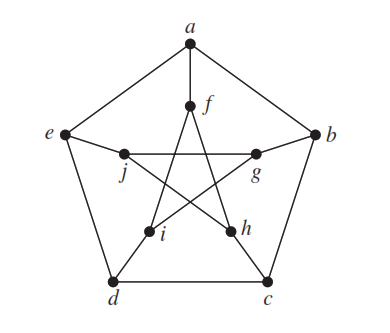
\includegraphics[width=0.5\linewidth]{img/petersen_graph.png}
	\caption{Rappresentazione grafica del grafo di Petersen}
	\label{fig:1}
\end{figure}

\subsection{Note}
\begin{itemize}
\item Con $opt(x)$ si intende il costo della soluzione ottimale, e non la soluzione ottimale stessa.
\item In questo corso, anche per semplicità, assumeremo che $P \neq NP$.
\item Le tecniche che andremo a vedere per risolvere problemi non vengono utilizzate solo per problemi complessi, ma anche, ad esempio per problemi polinomiali ma con input molto grandi.
\end{itemize}

\pagebreak
\section{Graph representations}
Vi sono diversi modi in cui si può decidere di rappresentare un grafo, ne vedremo alcuni, e noteremo come la scelta di una rappresentazione può essere migliore o peggiore a seconda delle caratteristiche del grafo che si vuole rappresentare.

\subsection{Adjacency list}
Tramite la lista di adiacenza si ha, per ogni vertice v tutti e soli i vertici w t.c. esista un arco da v a w, quindi, se si hanno n vertici e m archi, per memorizzare il grafo in memoria sarà necessario $\bigcirc(m)$; possiamo anche notare che, per verificare se è presente un arco tra due vertici sarà necessario $\bigcirc(\vert N(v) \vert)$, in quanto nel caso peggiore, il vertice che si vuole cercare è "l'ultimo" tra i vicini presenti nella lista di adiacenza del vertice di partenza, bisognerà quindi scorrere tutta la lista di adiacenza del vertice di partenza per trovare il vertice di arrivo.
\begin{figure}[h]
	\centering
	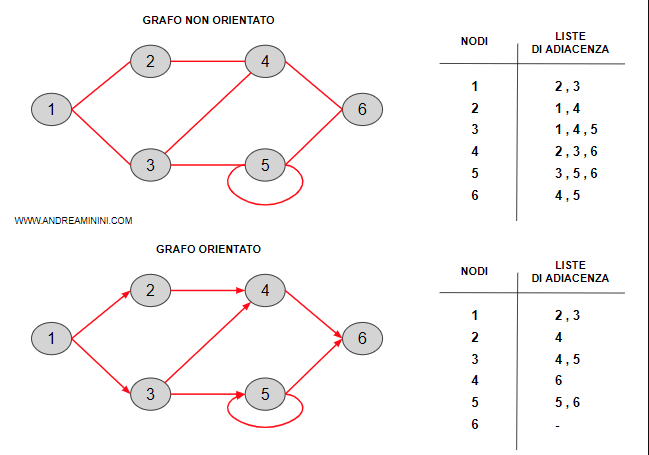
\includegraphics[width=0.7\linewidth]{img/lista_adiacenza}
	\caption{Rappresentazione grafica di una lista di adiacenza}
	\label{fig:2}
\end{figure}

\subsection{Adjacency matrix}
Tramite la matrice di adiacenza è possibile memorizzare un grafo tramite una matrice, dove gli indici delle righe e delle colonne sono i vertici, e, se vi è un arco dal vertice v al vertice w, allora alla riga v, colonna w troveremo un 1, altrimenti uno 0; è facile vedere che richiede $\bigcirc(n^{2})$ per essere memorizzata.
\begin{figure}[h]
	\centering
	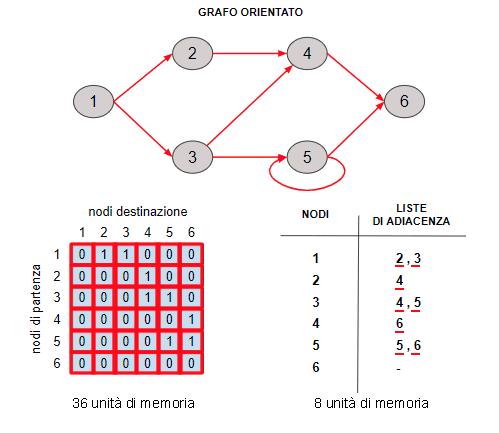
\includegraphics[width=0.7\linewidth]{img/matrice_adiacenza}
	\caption{Rappresentazione grafica di una matrice di adiacenza}
	\label{fig:3}
\end{figure}

\subsection{Incidence matrix}
La matrice di incidenza è un altro possibile modo per memorizzare un grafo in memoria, consiste in una matrice che ha come indici delle righe gli ID dei vertici e come indici delle colonne gli ID degli archi; è facile vedere che è necessario $\bigcirc(n * m)$ spazio per memorizzarla; in \ref{fig:4} possiamo vedere un esempio di matrice di incidenza.
\begin{figure}[h]
	\centering
	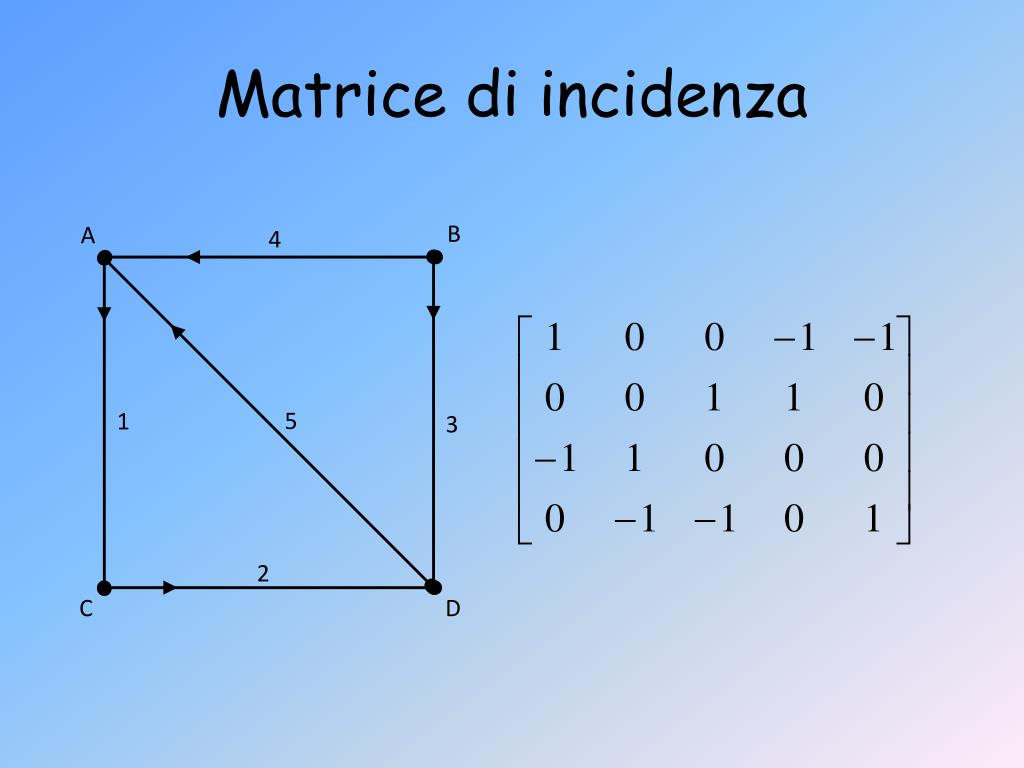
\includegraphics[width=0.7\linewidth]{img/matrice_incidenza.jpeg}
	\caption{Rappresentazione grafica di una matrice di incidenza}
	\label{fig:4}
\end{figure}

\subsection{Considerazioni sulle rappresentazioni}
Sapendo quindi che una lista di adiacenza richiede $\bigcirc(m)$, una matrice di adiacenza $\bigcirc(n^{2})$ ed una matrice di incidenza $\bigcirc(n * m)$, possiamo affermare quindi che:
\begin{itemize}
\item nel caso in cui si voglia memorizzare un grafo molto sparso, la struttura migliore tra quelle viste è la lista di adiacenza.
\item nel caso in cui il grafo che si vuole rappresentare ha un numero di archi molto alto, ossia con $m \simeq n$, allora vi è poca differenza tra lista di adiacenza e matrice di adiacenza.
\end{itemize}

\subsection{Considerazioni sugli algoritmi}
Un buon algoritmo deve avere una buona cache efficency, altrimenti, se occorrono molti miss, l'efficienza complessiva cala, possiamo affermare che tipicamente le strutture dati quali array hanno una buona cache efficency, a differenza degli alberi che hanno una scarsa cache efficiency.

\pagebreak
\section{Visite}

\subsection{DFS}
La depth-first search è un tipo di visita che prevede un vertice di partenza, detto radice (scelto casualmente), quindi si esplora il più lontano possibile ogni ramo prima di tornare indietro ad esplorare gli altri rami; richiede un tempo pari a $\bigcirc(\vert V \vert + \vert E \vert)$; utilizza una struttura di memoria detta pila(stack) per tenere traccia dei nodi scoperti durante l'esplorazione, per poi ritornare sui nodi non ancora esplorati.
\begin{figure}[h]
	\centering
	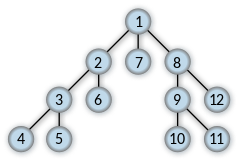
\includegraphics[width=0.7\linewidth]{img/Depth-first-tree.svg.png}
	\caption{ordine in cui vengono esplorati i vertici tramite depth first search}
	\label{fig:5}
\end{figure}

\subsection{BFS}
La breadth-first search, a differenza della depth-first, esplora prima tutti i nodi ad una certa profondità prima di passare alla profondità successiva; tipicamente si utilizza una struttura coda (queue) per tenere traccia dei nodi vicini che sono stati scoperti ma non ancora esplorati. Siccome nel caso peggiore si esploreranno tutti i vertici e tutti gli archi, la complessità in termini di tempo è pari a $\bigcirc(\vert V \vert + \vert E \vert)$. La BFS può essere utilizzata per trovare la distanza tra due vertici v e t, infatti, si può eseguire la BFS(v), quindi, una volta che arriva a t ci si ferma trovando così la distanza; questo procedimento introduce però un problema: l'exponential growth dei grafi, ossia che, se consideriamo un grafo G "classico", e consideriamo la cardinalità dei vertici di profondità pari a $n$ ossia $\vert n \vert$, allora in generale si può affermare che la cardinalità dei vertici di profondità pari a $n+1$ sarà circa ${\lbrace \vert n \vert \rbrace}^{2}$, quindi si può diminuire di molto lo spazio occupato in memoria effettuando due BFS: BFS(v) e BFS(t), quindi, quando si "incontrano", l'esecuzione termina e si può dedurre la distanza tra i due vertici sommando le due distanze.
\begin{figure}[h]
	\centering
	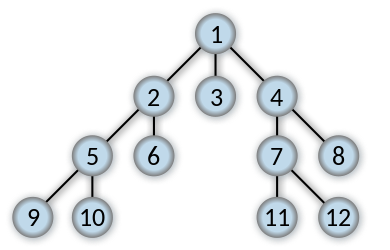
\includegraphics[width=0.7\linewidth]{img/Breadth-first-tree.svg.png}
	\caption{ordine in cui vengono esplorati i vertici tramite breatch first search}
	\label{fig:6}
\end{figure}

\subsection{Nota su DFS / BFS}
Siccome tipicamente vogliamo esplorare tutto un grafo, è bene considerare tutti i casi, un caso particolare da prendere in considerazione è quando il grafo da visitare è composto da più di una componente, questo, per come visitano il grafo BFS e DFS, implica che se si esegue una delle due visite sul grafo considerato, allora si esplorerà solo una delle componenti; quindi se si vuole esplorare interamente un grafo che ha, ad esempio, 5 componenti, si dovranno effettuare 5 visite (DFS o BFS che sia).

\pagebreak
\section{Problema - Shortest Path}
Shortest path è un problema sui grafi, richiede di trovare il cammino minimo tra due vertici s, t; è formulato come segue:
\begin{itemize}
\item Input
\begin{itemize}
\item Grafo $G = (V, E)$.
\item Funzione $w(v) \quad \forall v \in V$ che associa un peso ad ogni arco.
\item Due vertici $s, t$ tra i quali si vuole trovare lo shortest path.
\end{itemize}
\item Output: Uno shortest path di $G$ da $s$ a $t$, con shortest si intende un path che minimizza la somma dei pesi degli archi.
\end{itemize}

\subsection{Approccio - Dijkstra}
L'algoritmo di Dijkstra è un algoritmo per trovare il cammino minimo (shortest-path) tra vertici di un grafo pesato, ci sono più varianti dell'algoritmo, due di esse sono:
\begin{itemize}
\item L'originale: trovare lo shortest-path tra due vertici.

\item Trovare lo shortest-path tra un vertice (radice) e tutti gli altri vertici raggiungibili dal vertice radice. detto "shortest-path tree".
\end{itemize}
L'algoritmo originale di Dijkstra eseguiva in tempo pari a $\Theta(n^{2})$

\begin{figure}[h]
	\centering
	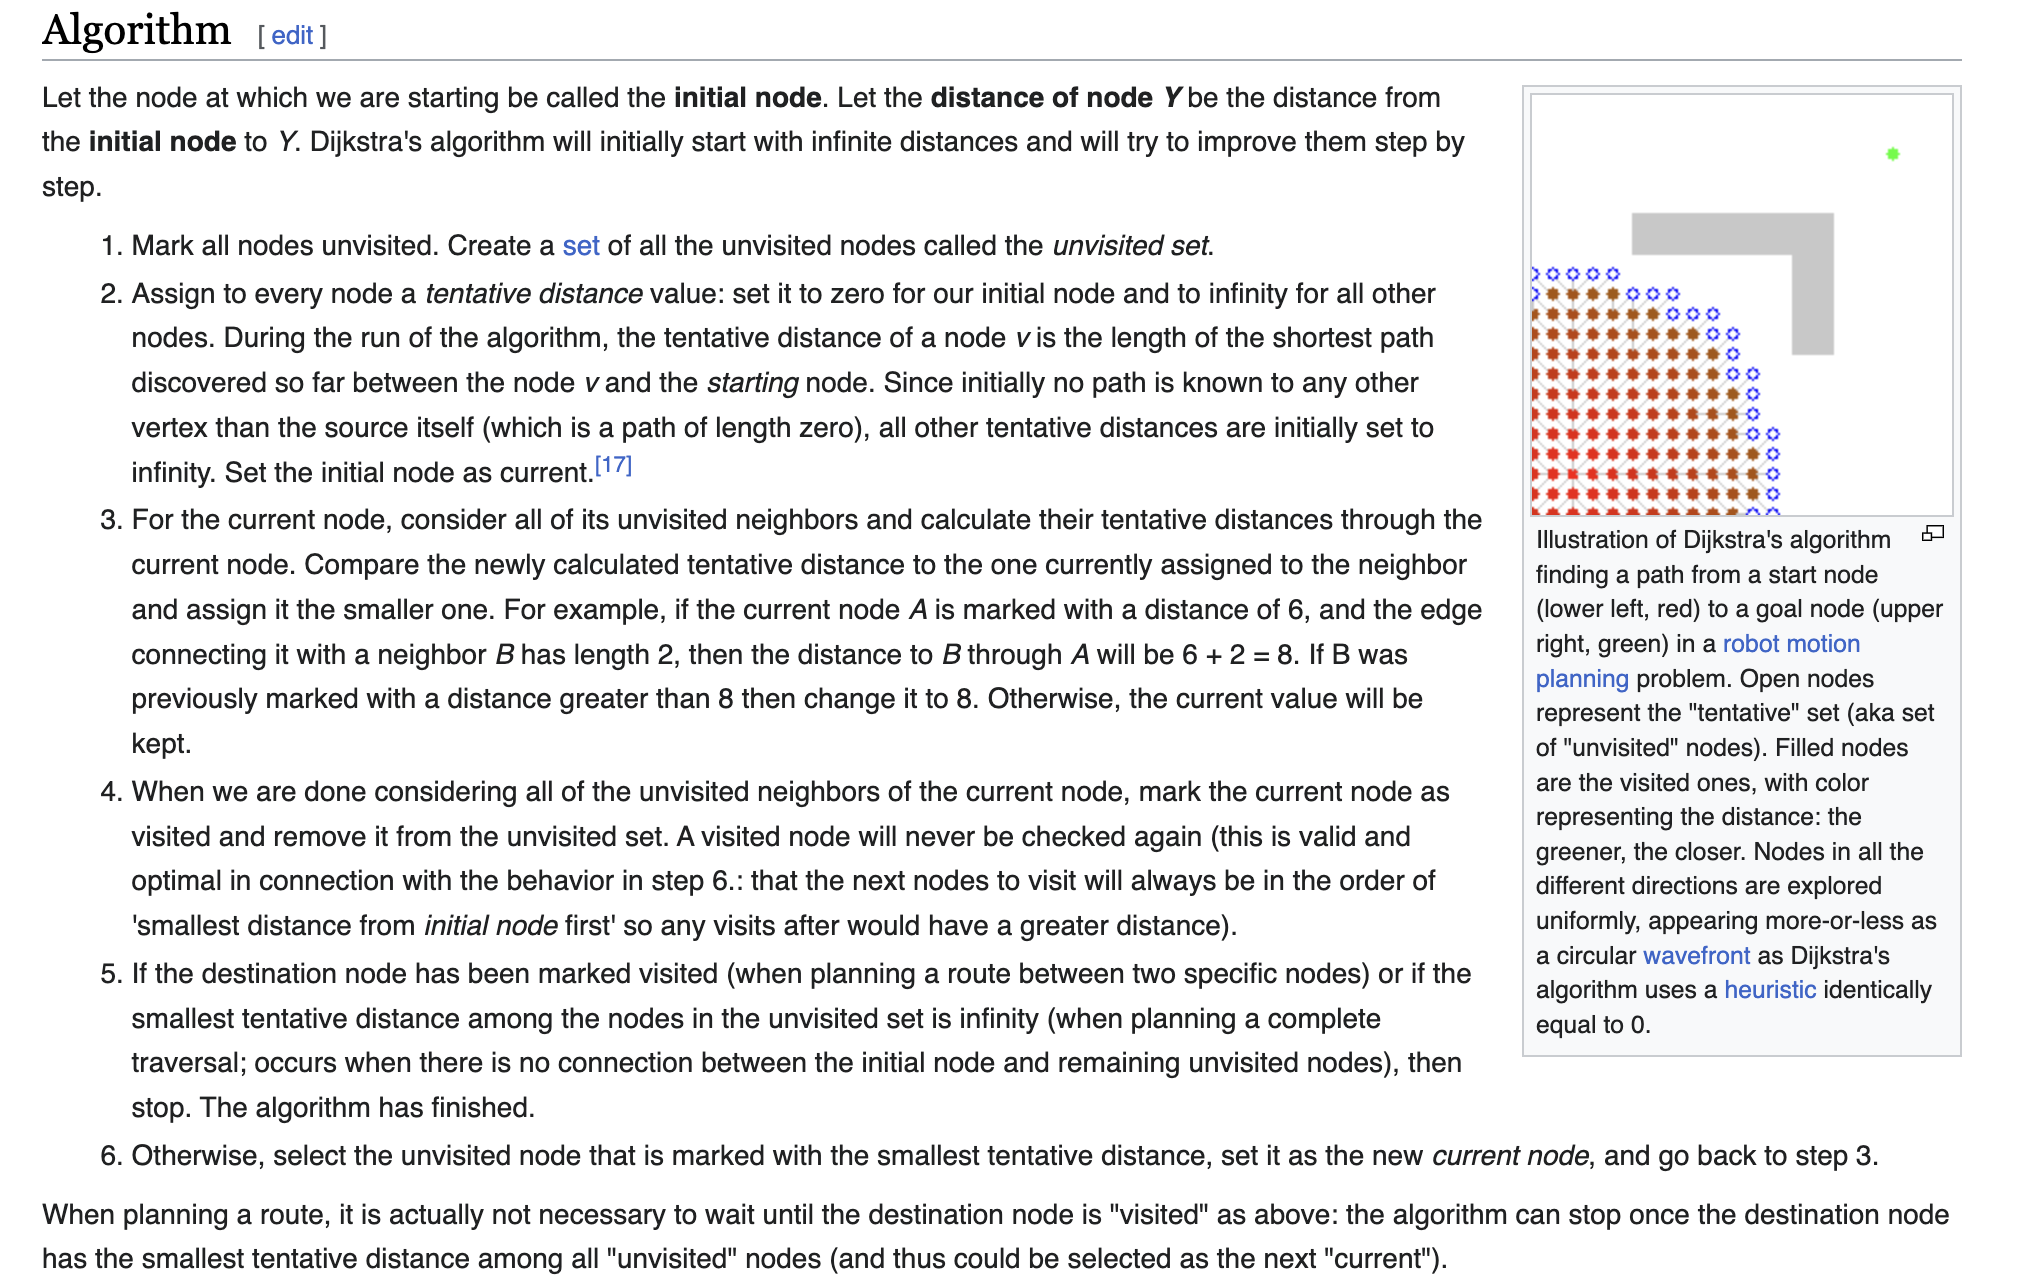
\includegraphics[width=0.9\linewidth]{img/Short_path}
	\caption{Descrizione dell'algoritmo di Dijkstra}
	\label{fig:Dijkstra algorithm}
\end{figure}

\subsection{Approccio - A*}
L'algoritmo A*, come Dijkstra, è utilizzato per trovare lo shortest-path tra vertici, ma, a differenza di Dijkstra, con A* è possibile cercare lo shortest-path solo tra due vertici scelti, e non tra un vertice radice e tutti gli altri; questo è un compromesso da considerare quando si utilizza un "euristica per soluzione specifica" (ossia con un nodo di destinazione scelto). La differenza principale con Dijkstra è proprio il fatto che A* utilizza un'euristica, questo gli permette di arrivare alla soluzione in maniera più rapida, a patto che $h(v) \leq d(v, destination)$, dove $h(v)$ è la distanza stimata tra $v$ e $destination$ dall'euristica utilizzata $h$, e $d(v, destination)$ è la distanza reale tra v e la destinazione; h potrebbe essere la distanza euclidea.

\pagebreak
\section{Connected components \& others}

\subsection{Connected components}
Nota: questa nozione viene tipicamente usata per grafi non orientati. Una componente connessa di un grafo G è un sottografo G' tale che:
\begin{itemize}
\item Presi due qualsiasi vertici di G' allora sono connessi da un cammino.
\item Il sottografo G' non è connesso a nessun altro vertice del grafo G.
\end{itemize}
\begin{figure}[h]
	\centering
	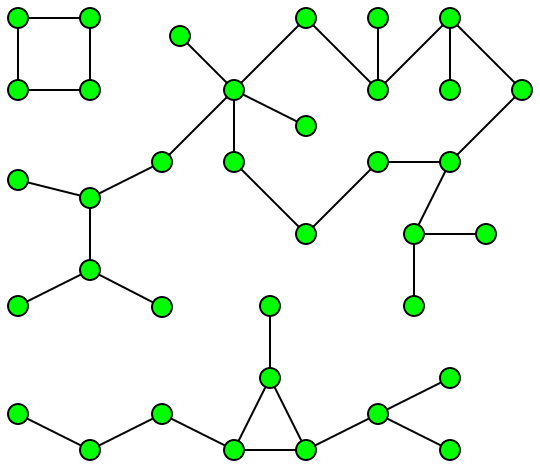
\includegraphics[width=0.5\linewidth]{img/conn_comp.png}
	\caption{Esempio di grafo con 3 componenti connesse}
	\label{fig:7}
\end{figure}
Si noti che, nel caso in cui il grafo $G$ è connesso, allora si ha una sola componente connessa: il grafo stesso.

\subsection{Strongly connected components}
Nota: la nozione di componente fortemente connessa è applicabile solo ai grafi orientati.
Considerando un grafo orientato $G = (V, E)$, esso è detto fortemente connesso se ogni vertice è raggiungibile da ogni altro vertice (notare che è diverso dal dire che il grafo sia completo, infatti ciò richiede che per ogni coppia di vertici vi sia un arco che li colleghi).

Quindi si dirà che una componente connessa del grafo è una componente fortemente connessa se, per ogni vertice di essa, se, per ogni coppia di vertici della componente, esiste una cammino tra i due, si noti che la componente deve essere un sottoinsieme massimale del grafo.
\begin{figure}[h]
	\centering
	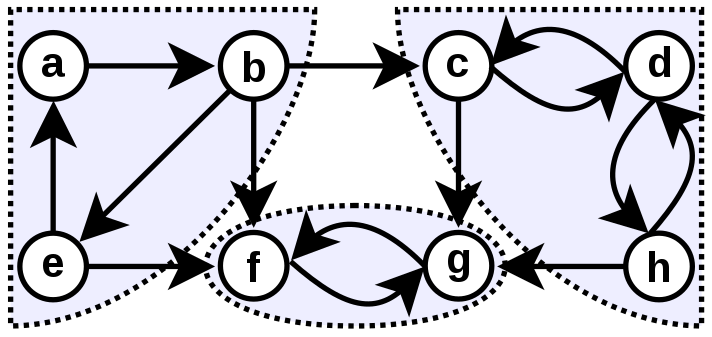
\includegraphics[width=0.5\linewidth]{img/Scc-1.svg.png}
	\caption{Un grafo viene suddiviso in componenti fortemente connesse, notare che il grafo è orientato, infatti la nozione di componente fortemente connesse è applicabile solo a grafi orientati}
	\label{fig:scc}
\end{figure}

\subsubsection{Approccio - Kosaraju}
Kosaraju è un algoritmo per trovare le componenti fortemente connesse in un grafo, l'idea fondamentale di questo algoritmo  è di utilizzare il fatto che il grafo trasposto (il grafo originale con il verso degli archi invertiti) ha le stesse scc del grafo originale. Vediamo quindi i passi dell'algoritmo:
\begin{itemize}
\item Si segnano tutti i vertici come unvisited.
\item Si dichiara una pila vuota S.
\item Si effettua una DFS a partire da un qualsiasi vertice v.
\item Ogni volta che si finisce di visitare un vertice v, allora si effettua push(v, S).
\item Si considera ora il grafo trasposto.
\item Si effettua v = pop(S)
\item Si effettua una DFS(v), quindi ogni volta che si attraversa un vertice che non è ancora stato visitato, lo si aggiunge all'attuale componente connessa.
\item Si ritornano le varie componenti connesse.
\end{itemize}
Nota: la pila viene utilizzata per tenere traccia dell'ordine con cui i vertici vengono esplorati, infatti troveremo in cima alla pila l'ultimo vertice esplorato di una certa componente connessa, quindi si effettuerà la pop proprio a partire da quello stesso vertice.

\subsubsection{Approccio - Path-Based}
Anche questo è un algoritmo per trovare le componenti fortemente connesse in un grafo G, anche questo, come Kosaraju utilizza la DFS, ma fa un solo passaggio invece di due.

Questo algoritmo utilizza due stack:
\begin{itemize}
\item Un prima pila in cui vi sono i vertici che non sono ancora stati assegnati ad una SCC.
\item Una seconda pila in cui vi sono dei vertici di cui ancora non si è determinato se appartengono a SCC diverse.
\end{itemize}

\subsection{Weak connected components}
Una componente debolmente connessa è una componente connessa nel grafo non-orientato sottostante; questa nozione è poco importante.

\subsection{Componenti k-vertici-connesse}
Una componente è $k$ connessa se ha più di k vertici ($\vert V \vert > k$) e se, rimuovendo al massimo un numero di vertici inferiore a k la componente continua a rimanere connessa.

Nota: se $k=2$ la componente viene anche detta \textit{biconnected component} oppure \textit{2-vertex-connected component}.

\begin{figure}[h]
	\centering
	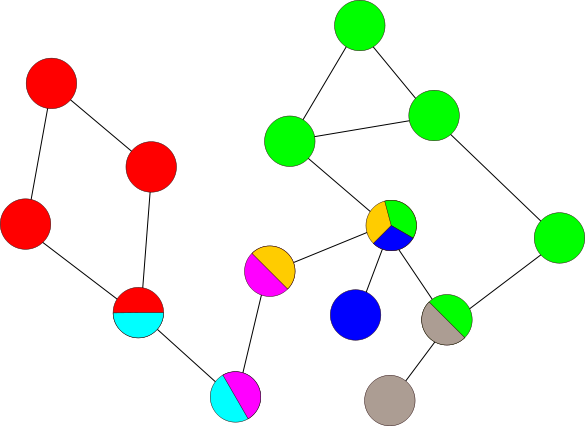
\includegraphics[width=0.5\linewidth]{img/Graph-Biconn-Comp.svg.png}
	\caption{Un grafo suddiviso nelle varie 2-connected components, i vertici che hanno più di un colore sono gli articulation point}
	\label{fig:2-conn-comp}
\end{figure}

\subsection{Componenti 2-lati-connesse}
Si dice che una componente è 2-edge-connected se rimuovendo un qualsiasi lato, allora la componente rimane connessa.

\subsubsection{Block graph}
Sia $G = \langle V, E \rangle$ un grafo connesso e non orientato, allora il block graph di G, chiamato $B = (W, F)$ tale che:
\begin{itemize}
\item $W = \lbrace$ componenti 2-conn di G $\rbrace \cup \lbrace$ artic. point di G $\rbrace$
\item $F = \lbrace (C, v)$ dove C è una comp. 2-conn di G, v un art. point t.c. $v \in C\rbrace$
\end{itemize}

\subsubsection{Block tree}
Sia $G = \langle V, E \rangle$ un grafo connesso e non orientato, allora il block tree di G, chiamato $B = (W, F)$ tale che:
\begin{itemize}
\item $W = \lbrace$ componenti 2-conn di G $\rbrace \cup \lbrace$ artic. point di G $\rbrace$
\item $F = \lbrace (C, v)$ dove C è una comp. 2-conn di G, v un art. point t.c. $v \in C\rbrace$
\end{itemize}

\subsubsection{Articulation point}
Gli articulation point sono importanti in quanto se ne viene rimosso uno qualsiasi, il numero di componenti connesse del grafo aumenta; ossia sono quei vertici che connettono almeno due componenti connesse. Più formalmente un vertice v è un articulation point se esiste un figlio w di v tale che:
\begin{itemize}
\item lowpoint(w) $\geqslant$ depth(v).
\item oppure
\item v è la radice del dft e v ha almeno due vertici figli.
\end{itemize}

\subsubsection{Lowpoint(v)}
Lowpoint: il lowpoint di un vertice v (lowpoint(v)) è la minima profondità raggiungibile dai discendenti o figli di v, v compreso; l'algoritmo utilizzato è un algoritmo ricorsivo bottom-up, in quanto l'algoritmo naive per il calcolo del lowpoint è invece molto inefficiente. L'algoritmo esegue una DFS del grafo dato, quindi, il lowpoint di un vertice v sarà:

$lowpoint(v) = min$
\begin{equation}
    \begin{cases}
      depth(v)\\
      min_{w \in N(v) \wedge w \notin par(v)} \lbrace depth(w) \rbrace\\
      min_{c \in children(v)} \lbrace lowpoint(c) \rbrace
    \end{cases}
\end{equation}

\subsection{L(v) e H(v)}
Definiamo quindi $L(v)$ e $H(v)$ come il minore/maggior valore di un etichetta di un discendente/ascendente di $v$ senza attraversare l'arco che connette $v$ ed il suo nodo genitore/figlio (un altro modo per dirlo è che bisogna rispettare l'ordine in cui i vertici vengono scoperti). Vediamo ora la definizione ricorsiva di $L(v)$ che viene sempre applicata ad una DFS:

$L(v) = min$
\begin{equation}
    \begin{cases}
      depth(v)\\
      min_{w \in N(v) \wedge w \notin par(v)} \lbrace depth(w) \rbrace\\
      min_{c \in children(v)} \lbrace L(c) \rbrace
    \end{cases}
\end{equation}
$$L(v) = min \lbrace depth(c)_{c \in children(v)} x_{x \in N(v) \setminus \lbrace v \rbrace} , w \rbrace$$
Il calcolo di $H(v)$ è invece più semplice, basta infatti contare il numero di discendenti di $v$ ($ND(v)$) quindi sottrarre 1 (tutto ciò sempre considerando la DFS):
$$H(v) = ND(v) - 1$$

\subsection{Archi bridges}
Un arco v di un grafo connesso è detto bridge se, rimuovendo v, allora il grafo non è più connesso; ossia se, rimuovendo l'arco bridge, il numero di componenti connesse del grafo aumenta. Utilizzando le definizioni che abbiamo appena dato di $L(v)$ e $H(v)$, possiamo affermare che un arco $v$ è bridge se e solo se: $$( L(v) = v ) \wedge ( H(v) < v + ND(v) - 1 )$$ quindi, se anche una sola delle due condizioni è violata, allora l'arco non è sicuramente un bridge. Per trovare tutti gli archi bridge di un grafo, possiamo utilizzare la DFS, infatti, anche se essa non esplora necessariamente tutti gli archi del grafo, esplora sicuramente tutti gli archi bridge del grafo; possiamo identificare un arco bridge grazie alla seguente noione: \textit{un arco è bridge sse non è contenuto in alcuna chain.} Un grafo viene detto "bridgeless" se non contiene alcun arco bridge.
\begin{figure}[h]
	\centering
	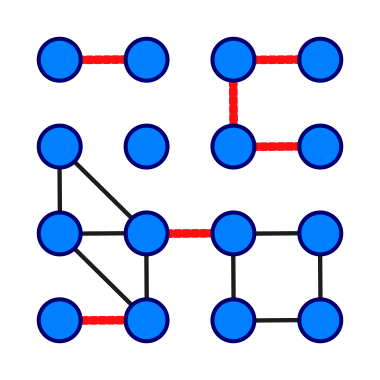
\includegraphics[width=0.5\linewidth]{img/Graph_cut_edges.svg.png}
	\caption{Rappresentazione grafica di alcuni archi bridge in rosso}
	\label{fig:1}
\end{figure}

\subsection{Approccio - Chain decomposition}
Chain decomposition è un algoritmo per trovare tutti gli archi bridge (e anche altre proprietà del grafo in analisi) tramite il DFS-tree, l'idea è di decomporre un grafo in un insieme di percorsi e cammini chiamati \textit{chain}, quindi:
\begin{itemize}
\item Si effettua una DFS (questo oltre a svolgere una visita, effettua anche un check implicito sulla connessione o meno del grafo).
\item Si ottiene quindi un albero-DFS $T$ con il vertice root $r$ (altrimenti si ferma).
\item La DFS assegna un \textit{Depth-first index (DFI)} ad ogni vertice.
\item Si assume quindi che gli archi di $T$ siano orientati verso $r$ (e sono quindi considerati backedges), e che quindi tutti gli archi di $G \setminus T$ siano nel verso opposto a $r$.
\item Si effettua la chain decomposition del grafo $G$.
\item Al termine, si potrà controllare quali vertici non fanno parte di alcuna chain, essi saranno gli archi bridges, possiamo affermare ciò grazie alla seguente nozione: \textit{se un arco $(v, w)$ non appartiene a nessuna chain, allora è un bridge.}
\end{itemize}

\begin{figure}[h]
	\centering
	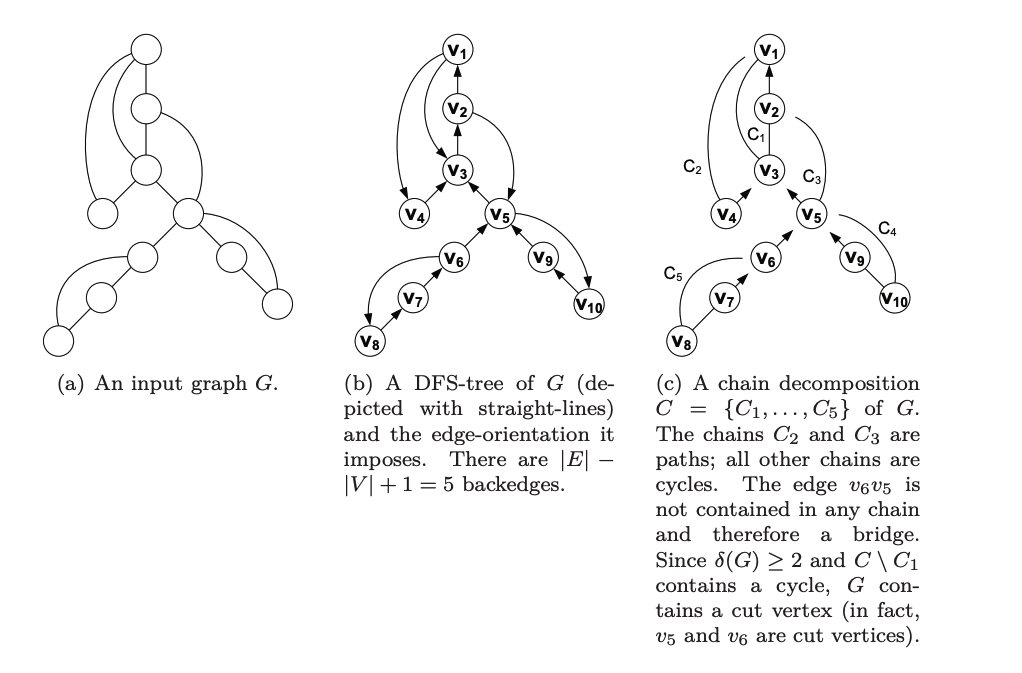
\includegraphics[width=1\linewidth]{img/chain_deco}
	\caption{Un grafo G, il DFS-tree di G, la chain decomposition di G}
	\label{fig:chain_deco}
\end{figure}

\subsection{Idea importante}
L'idea importante che viene utilizzata sia per trovare gli articulation point che per trovare i bridge, è che, nella DFS, una volta attraversato uno di essi non si sarà più in grado di tornare indietro.

\pagebreak
\part{Cuts and Flows}

\section{Problema - Max flow}
Max flow è un problema sui grafi (orientati) che richiede di trovare un flusso fattibile, facendo in modo che sia quello con capacità massima.

\begin{itemize}
\item Ogni arco è etichettato con la propria capacità (quante risorse possono passare per esso) $\forall (v, w) \in E \Rightarrow c(v, w)$.
\item Sappiamo quindi che un flusso $f$ relativo ad una arco $(v, w)$ sarà necessariamente $f(v, w) \leq c(v, w)$.
\item Va mantenuto il flow equilibrium: $\forall v \in V_{\setminus \lbrace s, t \rbrace} \sum_{u \in V} f(u, v) = \sum_{u \in V} f(v, u)$
\item Il flow in input alla sorgente deve essere nullo: $\sum_{u \in V} f(u, s) = 0$
\item Il flow in output dal target deve essere nullo: $\sum_{u \in V} f(t, u) = 0$
\item Quindi l'obiettivo del problema è: $max \sum_{v \in V} f(s, v) $
\end{itemize}

\begin{figure}[h]
	\centering
	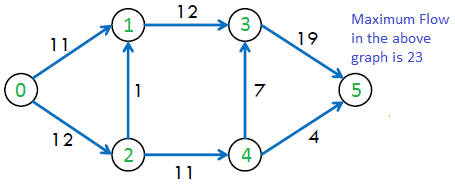
\includegraphics[width=0.7\linewidth]{img/ford_fulkerson2.png}
	\caption{Un grafo che rappresenta il problema max-flow}
	\label{fig:max flow graph}
\end{figure}

\subsection{Teorema Max-flow Min-cut}
Grazie a questo teorema, sappiamo che il max-flow da un vertice $s$ ad un vertice $t$ equivale alla capacità degli archi del min-cut del grafo dato.

\subsection{Approccio - Ford-Fulkerson}
È un algoritmo greedy per trovare il max-flow in una rete, fa utilizzo di due network: original network e residual network; consiste nel trovare ripetutamente un augmented path (ossia un path dalla sorgente alla destinazione, con della capacità residua su tutti gli archi del path stesso), utilizzare l'augmented path trovato, quindi aggiornare i due network e ripetere; tutto ciò si ripete fino a che non c'è più nessun path possibile.

Il residual network permette di "limitare quanto l'algoritmo è greedy", migliorando il risultato finale, e lo fa permettendo di ridurre il flusso precedentemente posto su un arco del grafo.

Si noti anche che la versione base di Ford-Fulkerson non garantisce la terminazione, infatti si potrebbe trovare una ripetizioni di augmented path che non terminano; è però da sottolineare che se termina, allora ritorna la soluzione ottima, questo è quindi un compromesso da considerare.

\begin{enumerate}
\item \url{https://www.youtube.com/watch?v=oHy3ddI9X3o}
\item \url{https://en.wikipedia.org/wiki/Ford%E2%80%93Fulkerson_algorithm}
\end{enumerate}

\subsubsection{Approccio - Edmonds-Karp}
L'algoritmo Edmonds-Karp è molto simile a Ford–Fulkerson (a volte viene anche considerato come un'estensione di esso), è infatti un'implementazione di esso, con la differenza che, in quest'ultimo viene definito l'ordine di ricerca degli augmented path; quindi è richiesto che il path trovato sia uno shortest path con capacità disponibile $> 0$ (quindi l'augmented path si trova tramite l'ausilio della BFS); si noti che la differenza principale tra Ford-Fulkerson ed Edmonds-Karp, è proprio il fatto che il secondo termina sempre, invece il primo non garantisce la terminazione.

\subsection{Approccio - Dinic}
Anche Dinic è un'algoritmo per trovare il max-flow $(s, t)$ in un grafo. Utilizza un level graph, ossia un grafo che, rispetto a quello iniziale:
\begin{enumerate}
\item Mantiene solo quegli archi che permettono di "avvicinarsi"(rispetto alla BFS) al vertice target, quindi un arco $(u, v)$ sarà nel level graph solo se $level(u) = k \wedge level(v) = k + 1$ (in sostanza vengono rimossi quegli archi all'indietro o laterali).
\item Possono far parte del level graph anche gli archi del residual graph, a patto che  rispettino il punto 1 e che abbiamo una capacità residua $>0$; si guardi figura \ref{fig:level graph} per capire meglio.
\end{enumerate}
\begin{figure}[h]
	\centering
	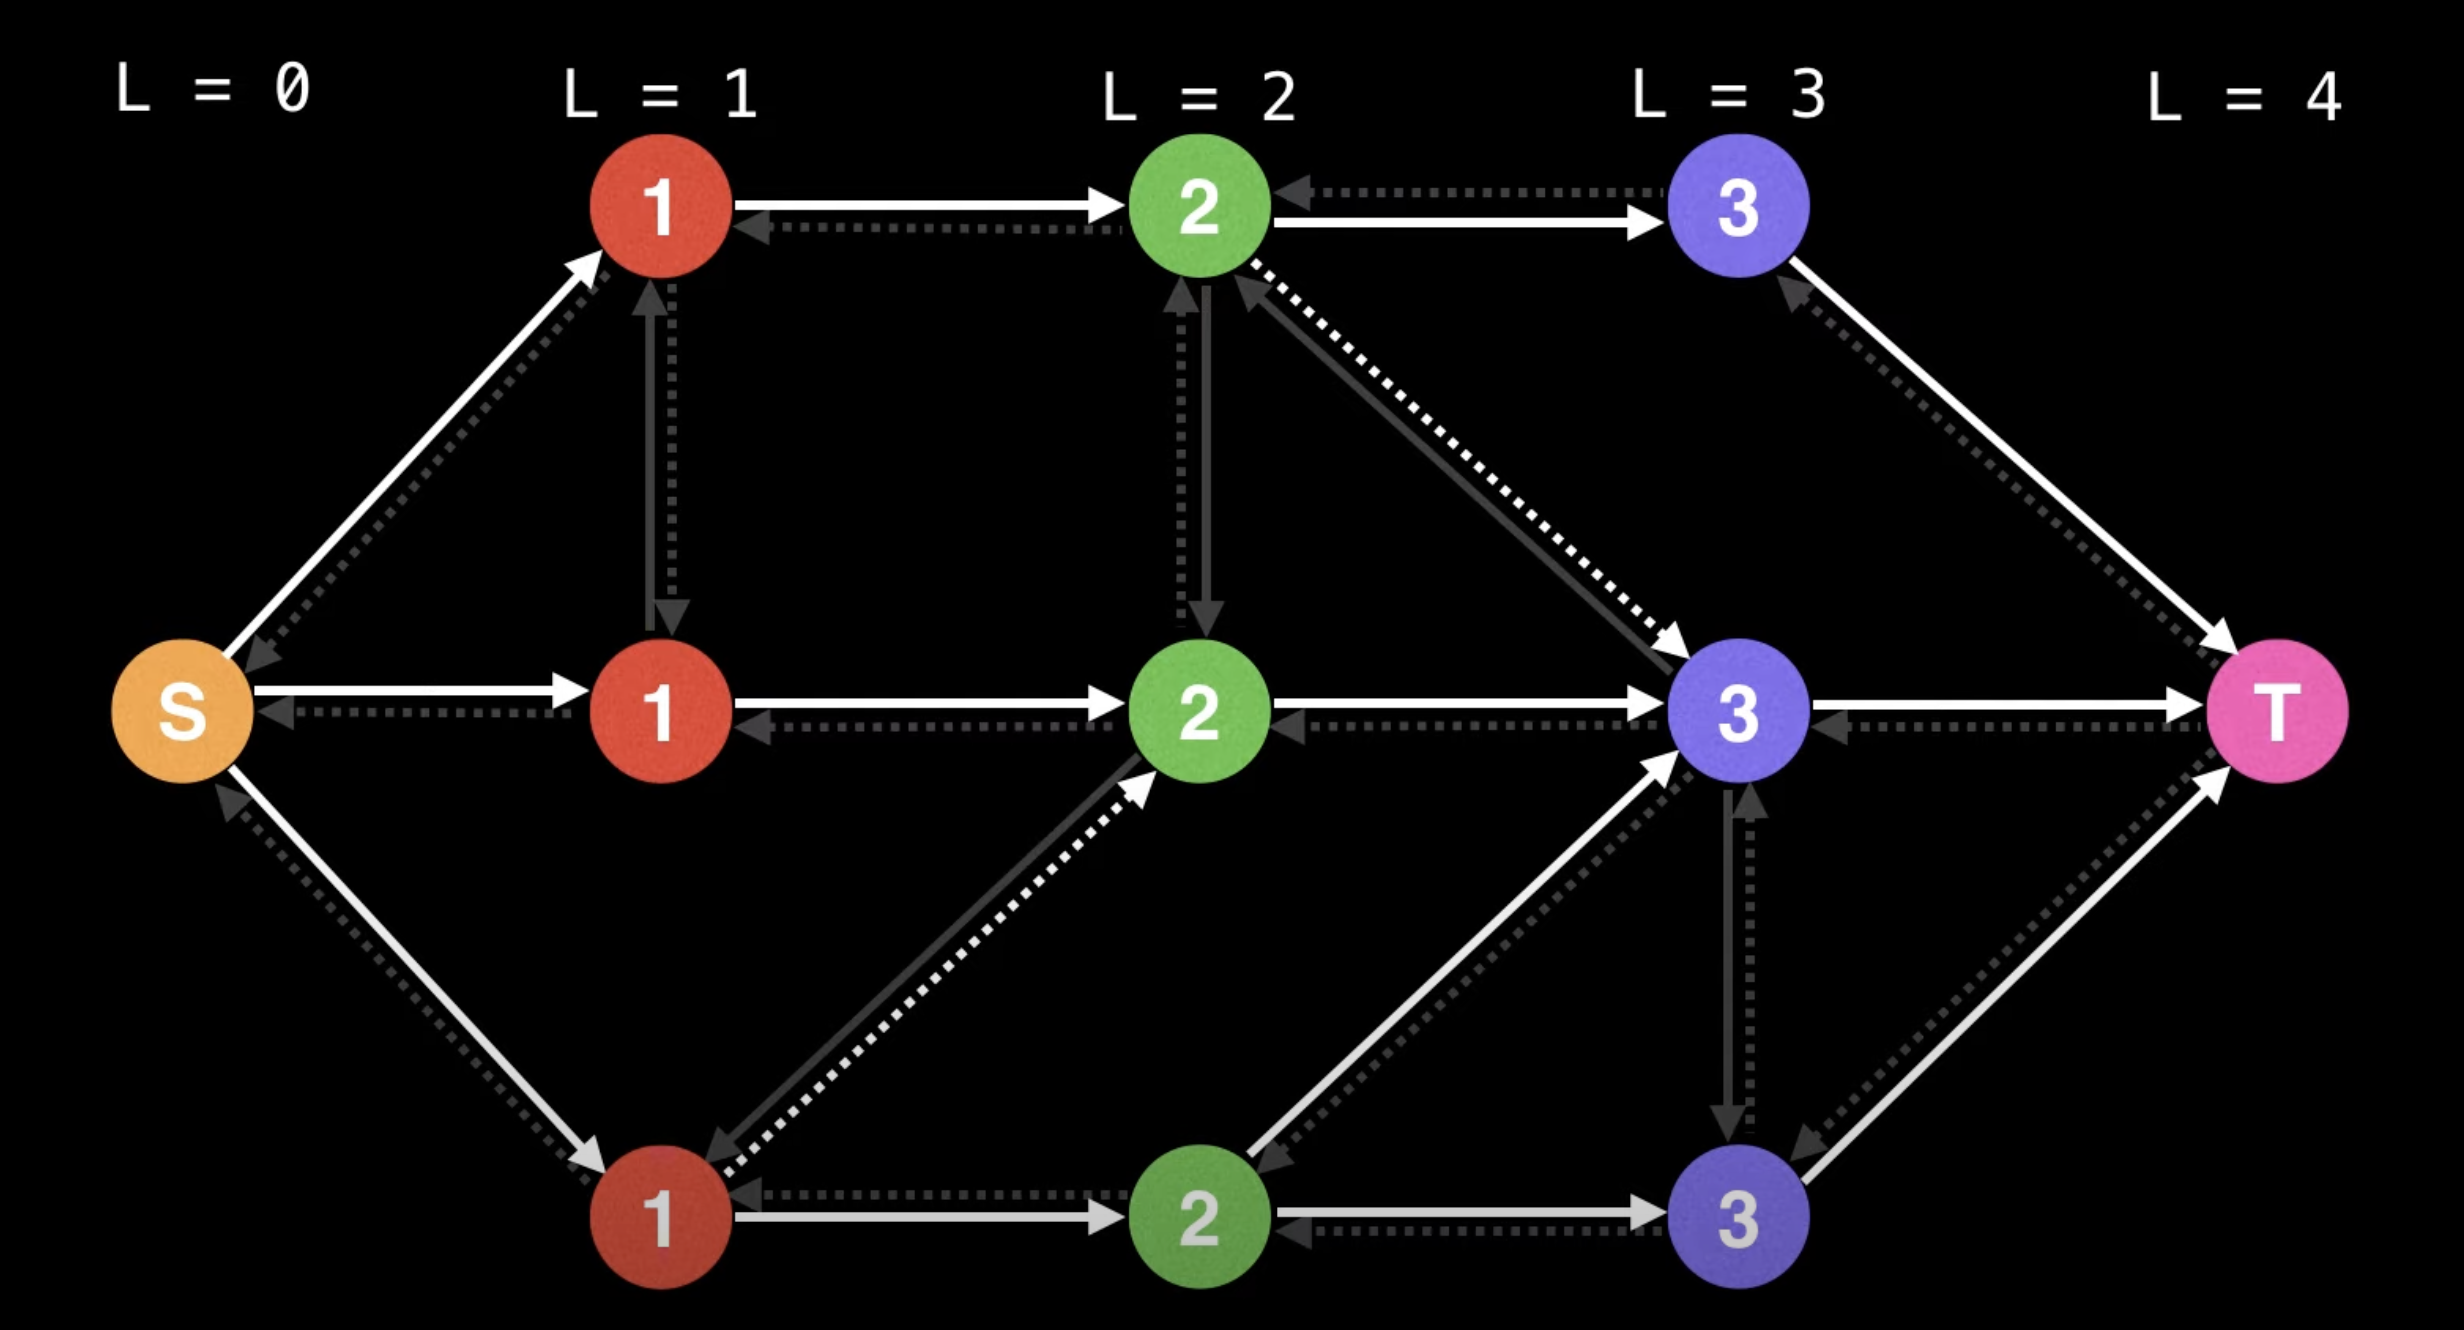
\includegraphics[width=0.7\linewidth]{img/lvl_graph.png}
	\caption{Gli archi grigi sono quelli esclusi dal level graph (quindi sono backward o sideways)}
	\label{fig:level graph}
\end{figure}
\textbf{I passi dell'algoritmo sono i seguenti:}
\begin{enumerate}
\item Effettuare $BFS(sorgente)$ per costruire il level graph.
\item Se il vertice destinazione non è stato raggiunto dalla BFS, allora si interrompe e si ritorna il max-flow.
\item While(! blocking flow):
\begin{enumerate}
\item Effettua $DFS(sorgente)$, ottenendo, se ne rimane almeno uno, un augmenting path.
\end{enumerate}
\item Aggiornare il grafo originale con i dati del blocking flow ottenuto.
\item Calcolo il level graph sul grafo originale aggiornato.
\item Se esiste un augmenting path nel level graph aggiornato, allora torno al punto 3; altrimenti calcolo la somma del flow dei blocking flow trovati durante le varie iterazioni e ritorno il valore calcolato.
\end{enumerate}

Fonti: \url{https://www.youtube.com/watch?v=M6cm8UeeziI}

\subsubsection{Considerazioni su Edmonds-Karp e Dinitz}
Edmonds-Karp richiede più iterazioni rispetto a Dinitz, ma ogni iterazione di Edmonds-Karp è meno costosa rispetto ad un iterazione di Dinitz; tipicamente si preferisce Dinitz tra i due.

\subsection{Approccio - Preflow-push}
Anche questo è un algoritmo per calcolare il max-flow di un dato network, si basa sull'idea di far scorrere il flusso da vertici più alti verso vertici più bassi, vedremo più avanti cosa si intende con alti o bassi; oltre a ciò, preflow-push ammette un disequilibrio del flow detto preflow: $$\forall v \in V \quad preflow(v)= \sum_{u \in V} f(u, v) \geq \sum_{w \in V} f(v, w)$$ ossia si permette, almeno momentaneamente, ad ogni vertice, di avere un flusso entrante maggiore o uguale a quello uscente, rompendo così l'equilibrio. Possiamo quindi definire un altro parametro, l'eccesso di flusso per un vertice v (excess of vertex): $$x(v) = \sum_{u \in V} f(u, v) - \sum_{w \in V} f(v, w)$$ Possiamo ora associare ad ogni vertice un altezza $(height(v))$; considerando in input il problema che richiede di trovare il maxflow dal vertice $s$ al vertice $t$, all'inizio avremo che i parametri saranno settati come segue:
\begin{itemize}
\item $height(s) = |V|$
\item $height(t) = 0$
\item $\forall v \in V_{\setminus \lbrace s,t \rbrace} \Rightarrow height(v) = 0$
\end{itemize}
I vertici $v$ con excess of vertex $x(v) > 0$ sono detti "attivi".

Vediamo ora alcuni approcci per alzare l'altezza dei vertici active, si noti che partiamo da questi in quanto sono i vertici che hanno un maggior flusso in ingresso rispetto a quello in uscita, quindi vogliono "liberarsi" del flusso in eccesso.
\begin{enumerate}
\item Considerando il grafo residuo, si alza del minimo necessario l'altezza dei vertici active: considerando un vertice active $v$, e $w$ l'insieme di vertici out-neihgbours di $v$, allora $$l(v) = 1 + min_{w \in V} \lbrace l(w) \rbrace$$
\item Il labelling è valido se $l(u) \leq l(v) + 1 \quad  \forall (u, v) \in$ {insieme degli archi del grafo residuo}
\item Si effettua la push da un vertice attivo $u$, verso un vertice $v$ con altezza inferiore, con esattamente questo vincolo : $l(u) = l(v) + 1$
\item Quando si effettua la push da $v$ a $w$, si inviano un numero di unità di flusso pari al minimo tra l'eccesso del vertice e la capacità residua del vertice uscente: $min \lbrace x(v), c(v, w) \rbrace $
\end{enumerate}
Durante i passi precedenti abbiamo affermato che all'inizio, l'altezza dei vertici, esclusi $s$ e $t$, viene posta pari a zero; questo rende utilizzabile l'algoritmo, ma una miglioria che si effettua tipicamente è di effettuare una backward BFS a partire da $t$, per calcolare l'altezza iniziale dei nodi; quindi, se si è in un caso fortunato, una volta effettuata la BFS, si potrà subito iniziare ad effettuare push, altrimenti si dovrà prima effettuare relabel su alcuni vertici. L'algoritmo può essere quindi considerato in due fasi: la prima, in cui si spinge il flusso in avanti, la seconda, in cui si rimanda alla sorgente tutto il flusso in eccesso, per ottenere il flow equilibrium.

\pagebreak
\section{Problema - Min-cut}
Min cut è un problema legato a max flow; dato un grafo $G$ non orientato, min cut richiede di trovare il minimum cut-set (e non un cut).

\subsection{cut(s, t)}
Un $cut(s, t)$ è un sottoinsieme $X \subseteq V$ tale che $s \in X, t \notin X$.

\subsection{cutset(s, t)}
Un $cutset(s, t) = C(S, T)$, dal vertice $s$ al vertice $t$ è un insieme di archi:
$$\lbrace (u, v) \in E \vert   u \in S \wedge v \in T\rbrace$$
ossia quegli archi che hanno un vertice che fa parte di $S$ ed il vertice opposto che fa parte di $T$. Possiamo notare che la rimozione degli archi nel $cutset(s, t)$ disconnetterà $s$ da $t$.

Si noti che abbiamo precedentemente definito gli archi bridge, ora possiamo dare un'altra definizione agli archi bridge: un arco bridge è un cutset composto da un solo arco.

\subsection{Approccio - Karger}
L'algoritmo di Karger si occupa di trovare un min cut dato un grafo, senza però fare distinzione tra i vari vertici, ossia non si assegna a due vertici il ruolo di sorgente e destinazione; l'idea su cui si basa questo algoritmo sono le contrazioni di un arco, ed utilizza questa idea proprio perché, statisticamente, è più probabile che sopravviva ad una contrazione un arco che fa parte del min-cut rispetto ad un arco che \textbf{non} ne fa parte. L'algoritmo è il seguente: Sia $G$ un grafo non orientato e senza pesi:
\begin{enumerate}
\item Prendere un arco random $(v, w)$.
\item Effettuare la contrazione del arco $(v, w)$.
\item Se rimangono solo due vertici ci si ferma, altrimenti si torna al punto 1.
\end{enumerate}
Tipicamente ritorna una soluzione che è molto vicina all'ottimo, ed è anche molto veloce; i vertici finali saranno i rappresentanti delle due partizioni del grafo. Una miglioria che è stata apportata a questo algoritmo (prendendo il nome di Karger-Stein) è di permettere di scegliere quando terminare, dove con "quando" si intende quanti vertici mancano alla terminazione, questo può portare ad una miglioria in quanto le ultime contrazioni sono responsabili di molti più vertici rispetto alle prime contrazioni.

\pagebreak
\part{Graph compression}

\section{Graph compression}
L'obiettivo della lossless graph compression è di minimizzare la memoria utilizzata per memorizzare il grafo senza perdere informazione.

Di seguito vedremo alcune tecniche per effettuare lossless graph compression sui grafi.

\subsection{Gzip}
L'idea della compressione Gzip è di processare un dato per trovare delle ripetizioni, quindi utilizzare queste ripetizioni per salvarle con tecniche particolari riducendo cosi la dimensione del dato finale; si è però notato con l'esperienza che queste ripetizioni non avvengono molto frequentemente nei grafi, quindi Gzip non è una buona tecnica per comprimere un grafo.

\subsection{Huffman coding}
Questa codifica è basata sulla probabilità di un simbolo di "apparire", quindi è necessario sapere a priori la probabilità di tutti i simboli, questa vincolo (downside) permette però di avere un codice ottimale, ossia che diminuisce al minimo la ridondanza.

Un'altra cosa da tenere in considerazione della codifica di Huffman è che è in grado di comprimere qualsiasi oggetto, indipendentemente da come esso è fatto.

\subsection{Elias gamma coding}
Questa codifica è solo per interi positivi dei quali non si conosce un upper bound a priori, richiede meno bit quando il numero da rappresentare è più piccolo; funziona nella seguente maniera, per codificare un numero $x \geq 1$:
\begin{enumerate}
\item Sia $N$ = $\lfloor log_{2} (x) \rfloor = 2^N \leq x < 2^{N+1}$.
\item La codifica è: $C$ = $N$ bit pari a $0$.
\item A $C$ si concatena la rappresentazione binaria di $x$.
\end{enumerate}
Quindi, per rappresentare un numero $x$, questa codifica richiede $2 \lfloor log_{2} (x) \rfloor + 1$ bit.
\begin{figure}[h]
	\centering
	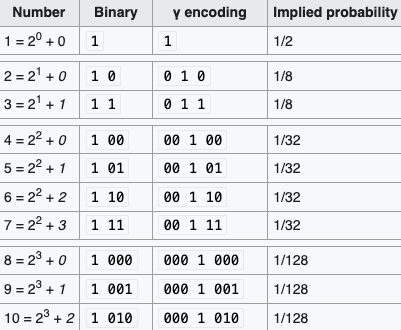
\includegraphics[width=0.5\linewidth]{img/elias_gamma}
	\caption{La rappresentazione dei primi 10 numeri tramite Elias gamma coding}
	\label{fig:elias_gamma}
\end{figure}


\subsection{Elias delta coding}
Anche questa codifica è solo per interi positivi dei quali non si conosce un upper bound a priori, richiede meno bit quando il numero da rappresentare è più piccolo; funziona nella seguente maniera, per codificare un numero $x \geq 1$:
\begin{enumerate}
\item Sia $N$ = $\lfloor log_{2} (x) \rfloor = 2^N \leq x < 2^{N+1}$.
\item Sia $L$ = $\lfloor log_{2} (N+1) \rfloor = 2^L \leq N+1 < 2^{L+1}$.
\item La codifica è: $C$ = $L$ bit pari a $0$.
\item Seguiti da la rappresentazione binaria del numero $N+1$ su $L+1$ bits.
\item Seguiti da la rappresentazione binaria di $x$ escluso il bit meno significativo.
\end{enumerate}
Quindi, per rappresentare un numero $x$, questa codifica richiede $$\lfloor log_{2} (x) \rfloor + 2 \lfloor log_{2} (\lfloor log_{2} (x) \rfloor + 1) \rfloor + 1 \quad bit$$
Si noti quindi che per interi molto grandi, è meglio utilizzare Elias delta al posto di Elias gamma, in quanto richiederà meno bit.
\begin{figure}[h]
	\centering
	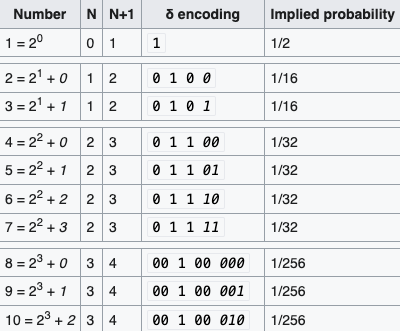
\includegraphics[width=0.5\linewidth]{img/elias_delta}
	\caption{La rappresentazione dei primi 10 numeri tramite Elias delta coding}
	\label{fig:elias_delta}
\end{figure}

\subsection{Run-length encoding}
In questa codifica, anche abbreviata con RLE, si cercano delle cosiddette "run" di un valore, ossia sequenze di un valore che si ripetono una successivamente all'altra, quindi vengono immagazzinate con la coppia (valore, numero di ripetizioni); queste run sono tipiche di dati quali immagini grafiche o disegni; per file che non contengono molte run, RLE potrebbe aumentare la dimensione del file; segue un esempio di RLE:
\begin{itemize}
\item Input: $AAAAAABBBB$
\item RLE encoding: $(A, 6)(B, 4)$
\end{itemize}

\subsection{Move-to-front transform}
L'idea di questa codifica è la seguente: ogni simbolo della sequenza viene rimpiazzato dal suo indice nella pila dei "simboli usati di recente", quindi:
\begin{itemize}
\item Una sequenza composta da $n$ simboli tutti uguali sarà rappresentata  da circa $n$ zeri.
\item Quando invece si incontra un simbolo che non veniva incontrato da molto tempo, allora sarà rimpiazzato da un numero molto grande.
\end{itemize}
\begin{figure}[h]
	\centering
	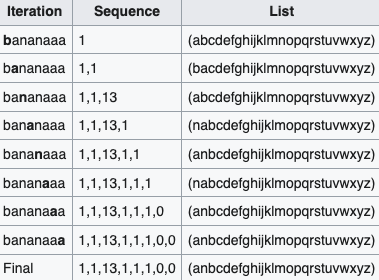
\includegraphics[width=0.5\linewidth]{img/move_front}
	\caption{La rappresentazione della sequenza "bananaaa" tramite move-to-front transform}
	\label{fig:move_front}
\end{figure}
Questa codifica è utile quando non si conoscono a priori la distribuzione delle frequenze e, nonostante ciò, permette di codificare i simboli più frequenti tramite sequenze di bit più corte.

\subsection{Variable length nibble code}
Questa codifica è solo per interi positivi dei quali non si conosce un upper bound a priori, funziona nella seguente maniera, per codificare un numero $x \geq 1$:
\begin{itemize}
\item Sia $p$ la rappresentazione binaria di $x$ con un aggiunta, a lato sinistro, di tanti 0 quanto basta per rendere la lunghezza di $p$ un multiplo di 3.
\item Dividere $p$ in blocchi di bit di lunghezza 3.
\item Aggiungere alla sx di ogni blocco uno 0.
\item Prendere il primo bit (quello più a sx) dell'ultimo blocco (che è uno 0 in quanto lo abbiamo aggiunto noi al passo precedente) e rimpiazzarlo con un 1.
\end{itemize}

\subsection{Minimal binary code}
Questa codifica è solo per interi positivi, dei quali si deve conoscere una stima dell'upper bound, funziona nella seguente maniera, per codificare un numero $0 \leq x \leq z - 1$:
\begin{itemize}
\item Sia $s = \lceil log_{2} (x) \rceil$.
\item Sia $p = s^s - z$.
\item Se $x < p$ si da in output la x-esima binary word di lunghezza $s - 1$.
\item Se $x \geq p$ si da in output la $(x - z + 2^s)$-esima word di lunghezza $s - 1$.
\end{itemize}
Questa codifica risulta ottimale se, presi tutti gli elementi che si trovano nel range dato, essi hanno tutti la stessa probabilità.

\subsection{Gap representation}
Questa rappresentazione è basata sull'assunzione che i vertici vicini ad un vertice $v$ abbiano un etichetta "vicina" a quella di $v$; quindi funziona nella seguente maniera: data la lista di adiacenza di un vertice $v$, ogni vertice è rappresentato tramite la differenza con il vertice precedente; vediamo un esempio della codifica tramite la figura \ref{fig:gap_repr}:
\begin{itemize}
\item Consideriamo il vertice 3.
\item La lista di adiacenza è: $adj(3) = \lbrace 1, 2, 4, 5 \rbrace$.
\item Il calcolo della rappresentazione è: $\lbrace 1-3=-2, 2-1=1, 4-2=2, 5-4=1 \rbrace$.
\item La rappresentazione finale è quindi: $\lbrace -2, 1, 2, 1 \rbrace$.
\end{itemize}

\begin{figure}[h]
	\centering
	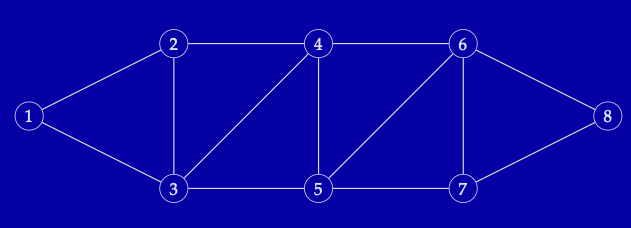
\includegraphics[width=0.8\linewidth]{img/gap_repr}
	\caption{un grafo di esempio}
	\label{fig:gap_repr}
\end{figure}

\subsection{Web graph}
Si noti che la tecnica di compressione di grafi più utilizzata è la \textit{web graph}, essa utilizza una combinazione delle tecniche che abbiamo visto fin'ora per ottimizzare il più possibile le dimensioni di grafi di grandi dimensioni, si chiama così proprio perché il web è in sostanza un grafo gigantesco.

\pagebreak
\part{Bipartite matching}

\section{Bipartite graphs}
Sia $G = (V, E)$ un grafo non diretto, G è detto grafo bipartito se esistono due subset $A, B$ di $V$:
\begin{itemize}
\item $A, B \subseteq V$
\item $B = V \setminus A$
\item $A = V \setminus B$
\item $E \cap (A \times A) = \emptyset$
\item $E \cap (B \times B) = \emptyset$
\end{itemize}
Ossia $A$ e $B$ sono tra loro \textbf{indipendenti} e \textbf{disgiunti}, quindi, ogni arco connette un vertice di $A$ ad un vertice di $B$; i due subset $A$ e $B$ di un grafo bipartito possono anche essere interpretati tramite il problema di graph coloring con due colori, ossia: per ogni arco, i due vertici che sono collegati ad esso devono avere due colori diversi.

Un modo per verificare se un grafo è bipartito è quello di controllare se contiene cicli di lunghezza dispari (questo significherebbe che c'è una arco all'interno dello stesso lato/partizione) e che quindi il grafo esaminato non è bipartito; al contrario, se non include nessun ciclo dispari, allora il grafo è bipartito.

\begin{figure}[h]
	\centering
	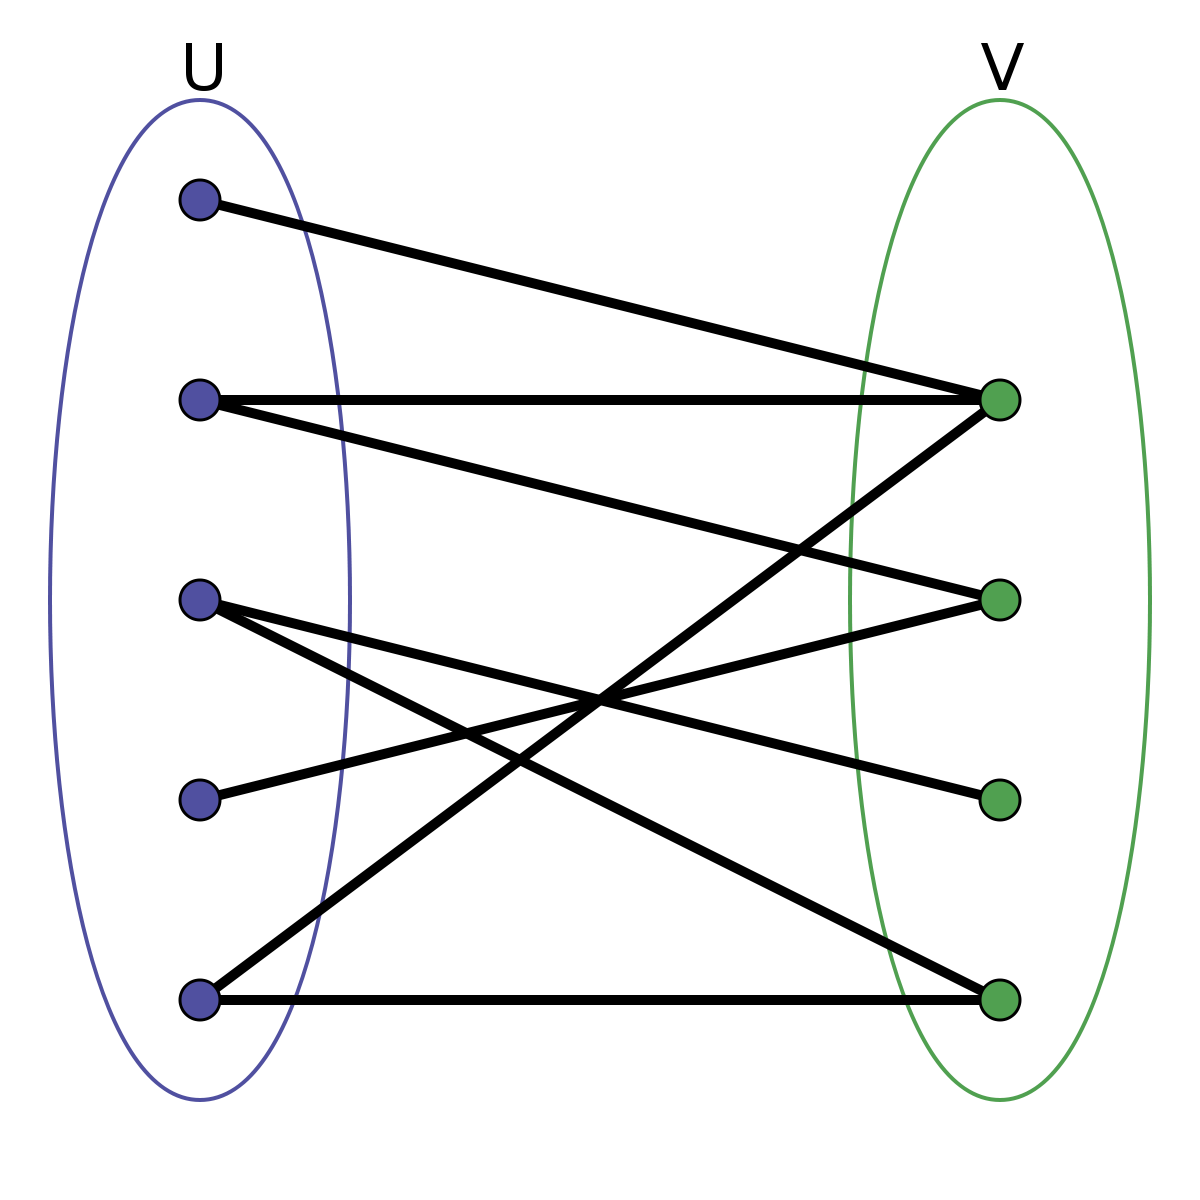
\includegraphics[width=0.6\linewidth]{img/bipartite-graph.png}
	\caption{Esempio di grafo bipartito, i due sottoinsiemi di V che lo compongono sono U e V, possiamo notare che U e V non hanno nemmeno un vertice in comune.}
	\label{fig:Esempio di grafo bipartito}
\end{figure}
\begin{figure}[h]
	\centering
	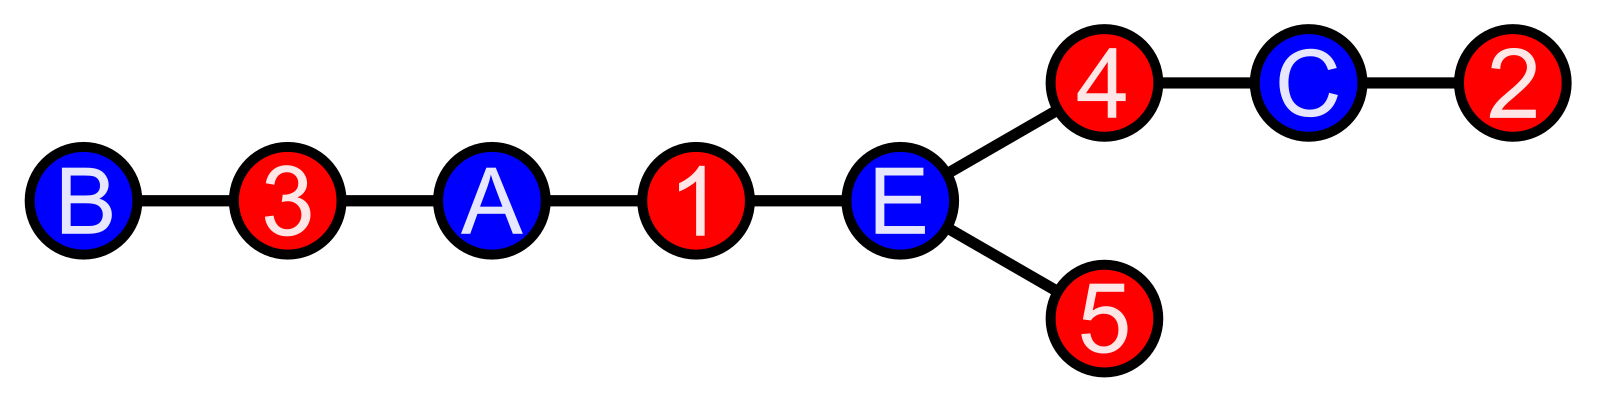
\includegraphics[width=0.6\linewidth]{img/Bipart_graph_no_cross.svg.png}
	\caption{Esempio di grafo bipartito,possiamo notare come sia possibile colorare ogni vertice di un certo colore, quindi il colore indicherà il subset di appartenenza del vertice.}
	\label{fig:Esempio di grafo bipartito senza incroci}
\end{figure}

\section{Matching}

\subsection{Matching in general graphs}
Sia $G = (V, E)$ un grafo non diretto, allora $M \subseteq E$ è matching se non esistono due archi di $M$ che condividono un vertice; si noti che si effettua una distinzione tra matching nei grafi classici e nei grafi bipartiti in quanto, nonostante esistano algoritmi polinomiali che risolvono matching nei grafi classici, esistono algoritmi ancora più efficienti per risolvere matching su grafi bipartiti (questa informazioni è importante soprattutto se fossimo interessati a risolvere matching solo su grafi bipartiti, cosa che spesso accade).

\subsection{Max cardinality matching in a bipartite graph}
Sia $G = (V, E)$ un grafo bipartito con le due partizioni: $A, B$, la formulazione ILP del problema è descritta in figura \ref{fig:max_card_match}, ossia si vuole ottenere il matching che ha il maggior numero possibile di archi al suo interno; Questo problema è risolvibile in maniera più efficiente su grafi bipartiti rispetto a grafi non bipartiti.

\subsubsection{Approccio - Flow network x max card matching}
Siccome abbiamo visto in precedenza (\url{https://www.youtube.com/watch?v=GhjwOiJ4SqU}) che l'approccio greedy per max cardinality matching non porta necessariamente all'ottimo, vogliamo utilizzare un altro approccio: si vuole quindi trasformare l'istanza del problema max card matching in un'istanza di flow network, risolvendo trovando il maximum flow:
\begin{itemize}
\item Le due partizione del grafo sono $A, B$.
\item $\forall (u, v) \in E$ rendere $(u, v)$ un arco diretto da $A$ a $B$.
\item $\forall (u, v) \in E$ aggiungere una capacità di $1$ unità.
\item Aggiungere un vertice sorgente $s$, $\forall v \in A$ aggiungere un arco $(s, v)$ (anch'esso orientato e con capacità $1$).
\item Aggiungere un vertice destinazione $t$, $\forall u \in B$ aggiungere un arco $(u, t)$ (anch'esso orientato e con capacità $1$).
\end{itemize}
Si potrà quindi eseguire un qualsiasi algoritmo per max flow (ad esempio Ford-Fulkerson), sull'istanza ottenuta, per trovare un maximum cardinality matching, quindi, gli archi con flusso pari a $1$ sono quelli che fanno parte del matching, tutti gli altri sono esclusi.

\subsection{Augmenting path in matching}
Un augmenting path del grafo dato è un path tale che:
\begin{itemize}
\item Inizia/finisce in un vertice che non è coperto dal matching.
\item Alterna archi che sono nel matching con archi che non sono nel matching.
\end{itemize}
Quindi si può affermare che:
\begin{itemize}
\item Se trovo un augmenting path, posso usarlo per migliorare il risultato.
\item Se non vi sono più augmenting path, allora il matching trovato è ottimale.
\end{itemize}


\begin{figure}[h]
	\centering
	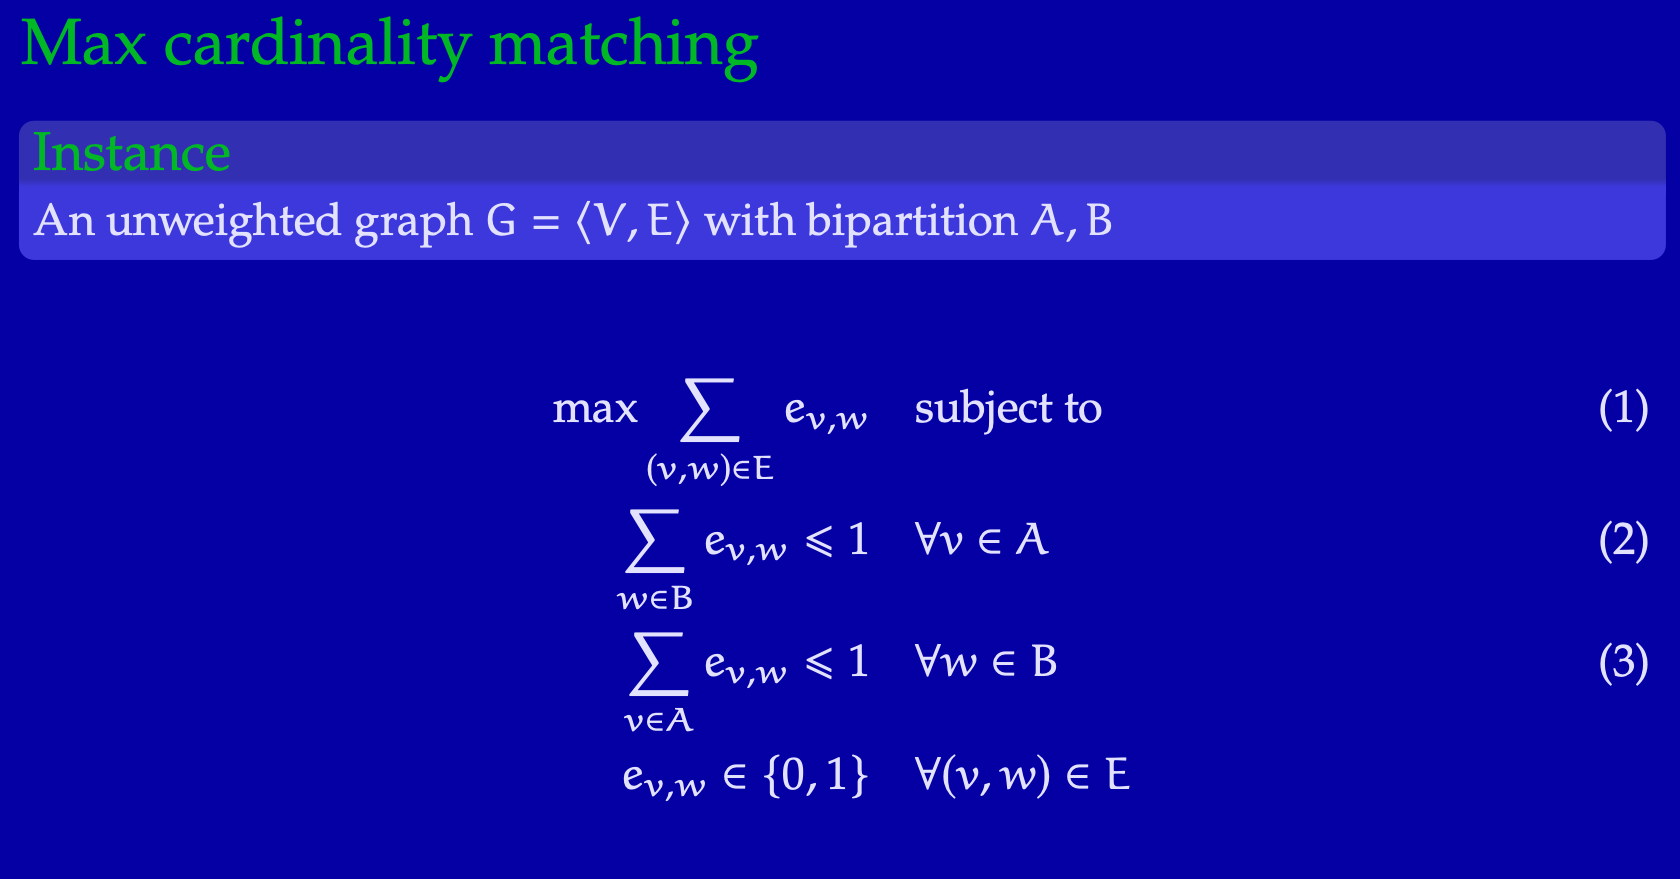
\includegraphics[width=0.8\linewidth]{img/max_card_match}
	\caption{Descrizione ILP del problema max cardinality matching in a bipartite graph.}
	\label{fig:max_card_match}
\end{figure}

\subsection{Perfect Matching}
\begin{itemize}
\item Input: grafo $G = (A \cup B, E)$ non diretto.
\item output: un maximun cardinality matching di $G$, che tocca tutti i vertici di $G$.
\end{itemize}

\subsection{Approccio - Hungarian}
Si noti che questo algoritmo è originariamente usato per risolvere il problema dell'assegnamento, ciò nonostante è facile trasformare un istanza di matching, nel caso di grafi bipartiti, in un istanza di assegnamento, vediamo quindi come formulare il problema in termini di grafi bipartiti:
\begin{itemize}
\item Input: un grafo $G = (S, T, E)$, dove $S$ sono i vertici che rappresentano i lavoratori, $T$ sono i vertici che rappresentano un lavoro, $E$ sono gli archi del grafo; ad ogni arco $e \in E$ viene associato un costo non negativo $c(i, j)$.
\item Output: un perfect matching di $G$ con costo minimo (lo si ottiene in tempo polinomiale).
\end{itemize}
Passi dell'algoritmo:
\begin{itemize}
\item Sia $y:(S \cup T) \rightarrow R$ una funzione chiamata \textit{potenziale} se $y(i) + y(j) \leq c(i, j) \quad \forall \quad i \in S, j \in T$, quindi, il valore della funzione potenziale $y$ è uguale alla somma del potenziale di tutti i vertici: $\displaystyle\sum_{v \in (S \cup T)} y(v)$.
\end{itemize}
Questo metodo trova un perfect matching ed un potenziale tali che il costo del perfect matching è pari al valore del potenziale, questo implica che entrambi sono ottimali (minimum-cost perfect-matching); si noti che questo algoritmo trova un perfect matching per archi che sono detti \textit{thight edges} (un arco $(i, j )$ è detto \textit{tight} per un potenziale $y$ se $y(i) + y(j) = c(i, j)$).

\pagebreak
\part{Coloring}

\section{Problema - Graph coloring}
Graph coloring è un altro problema che riguarda i grafi, è importante in quanto, come SAT, viene studiato da molti anni, essendo presente nei \textit{21 problemi NP-completi di Karp}; ne esistono diverse varianti, la più semplice richiede di: dato un grafo, una funzione che assegna un colore ad ogni vertice del grafo, trovare il minimo numero di colori tali che, per ogni arco del grafo, i suoi due vertici hanno colore diverso; questo problema è anche detto, più precisamente \textit{vertex-coloring}.

Più formalmente, graph-coloring (vertex-coloring) è:
\begin{itemize}
\item Input
\begin{itemize}
\item Grafo $G = (V, E)$
\item funzione di colorazione $\lambda$ t.c. $\forall v \in V \quad \lambda(v) =$ colore di $v$ 
\end{itemize}

\item Output
\begin{itemize}
\item Il minimo numero di colori utilizzabili tali che: $$\forall (v, u) \in E \quad \lambda(v) \neq \lambda(u)$$
\end{itemize}
\end{itemize}

Graph coloring è un problema che contiene diverse varianti, alcune di esse sono:
\begin{itemize}
\item Vertex-coloring: vengono colorati i vertici, questa è la variante più classica e semplice.
\item Edge-coloring: vengono colorati gli archi al posto dei vertici.
\item Proper coloring: dove viene richiesto che effettivamente, per ogni arco del grafo, esso abbia ai due estremi due vertici di colori diversi; quindi ci sono altre varianti che ammettono alcuni archi con ai due sestremi lo stesso colore.
\item Complete coloring: dove viene richiesto che, dato un grafo, tutti i vertici siano effettivamente colorati; quindi ci sono altre varianti che ammettono la possibilità di avere dei vertici lasciati "uncolored".
\end{itemize}

\subsubsection{Relazione con Clique}
Considerando il problema k-clique, sappiamo che esso indica che c'è un sottografo $G'$ di $G$ tale che $G'$ è completo, questo implicherà che, se si vuole colorare il suddetto grafo, si dovranno necessariamente utilizzare almeno k colori.

\subsection{Riduzione del input}
Una pratica da tenere in considerazione in coloring è la riduzione della dimensione dell'input:
\begin{itemize}
\item \textbf{Adjacent to all vertices}: se si considera una vertice che è adiacente a tutti gli altri vertici del grafo, allora sicuramente dovrò utilizzare un nuovo colore per esso, quindi, quando inizio a risolvere il problema, posso controllare se esistono dei vertici $x$ con questa proprietà, quindi li si rimuove dal grafo, si risolve coloring sul grafo senza i vertici $x$, quindi si prende la soluzione e si aggiungono di nuovo i verti $x$, assegnando ad ognuno di loro un nuovo colore.
\item \textbf{Included Neighborhood}: trovo due vertici $v, u$ t.c. $N(v) \subseteq N(u)$, allora li si può rimuovere dal grafo $G$ ottenendo $G'$, eseguire coloring sul grafo $G'$, quindi aggiungere al risultato di coloring su  $G'$ $v$ e $u$ colorandoli dello stesso colore.
\item \textbf{Articulation point}: si considera un articulation point $x$ che collega due componenti $c1, c2$ del grafo $G$, allora possiamo risolvere coloring su $c1 \cup x$ e $c2 \cup x$, si noti che i due risultati potrebbero avere assegnato un colore diverso a $x$, ma questo non importa, in quanto i colori possono essere permutati a piacimento, quindi facendo risultare sia per $c1$ che per $c2$ lo stesso colore di $x$.
\item \textbf{Separating clique}: è una versione più generica della regola precedente, quindi si considera un k-separating clique (sappiamo che per esso dovremo utilizzare esattamente k colori), che collega due componenti $c1$, $c2$, quindi poi si risolverà come nella regola precedente; si noti che cercare un \textit{k-separating-clique} equivalente a cercare una \textit{k+1-connected-component}.
\end{itemize}

\subsection{Approccio - ILP}
Nella formulazione ILP di vertex coloring che ha mostrato alla lavagna, il prof ci ha fatto notare che una possibile miglioria poteva essere di aggiungere un altro vincolo: $u_i \geq u_{i+1}$ ossia che il primo colore sarà quello a cui viene assegnato il numero maggiore di vertici, e così a calare.

\subsection{Approccio - Greedy}
Abbiamo visto un algoritmo greedy per vertex-coloring, questo funziona come segue:
\begin{itemize}
\item Si considerano i vertici con un determinato ordine, (anche casuale): $v_1, v_2, ... , v_i$
\item Si parte del primo vertice, quindi, per ogni vertice gli si assegna il più piccolo colore disponibile, ossia che non sia assegnato a nessuno dei suoi vicini.
\end{itemize}
Nota: esiste un ordinamento per il quale questo algoritmo ritorna la soluzione ottimale.

Il prof ha commentato dicendo che greedy è buono in quanto è veloce, anche se non sempre ritorna la soluzione ottimale.

\subsection{Approccio - Welsh Powell}
Anche questo è un algoritmo greedy, che però cerca di migliorare la versione sopra, infatti in questo caso, l'ordinamento dei vertici non è casuale: i vertici vengono ordinati in base al loro grado; questo garantisce che vengano utilizzato al massimo un numero di colori pari al massimo grado del grafo + 1.

\subsection{Approccio - Iterated greedy}
L'idea di questo algoritmo è la seguente:
\begin{enumerate}
\item Si prende l'ouput $x$ dell'algoritmo greedy.
\item Si riordinano i vertici di $x$ secondo un qualche criterio.
\item Si esegue di nuovo l'algoritmo greedy utilizzando come ordinamento quello calcolato al punto 2.
\end{enumerate}
Alcuni possibili criteri sono: Largest class first; invertire le classi dell'input; riordinamento random.

\subsection{Approccio - DSatur}
É un altro approccio, simili a quello greedy, però, in questo caso, i vertici vengono colorati secondo il seguente ordine: si considerano tutti i vertici che sono ancora da colorare, quindi tra questi, si prende quello che ha la saturazione massima, dove con saturazione si intende il numero di colori distinti che sono assegnati ai vicini del vertice considerato. in caso vi siano due vertici con saturazione massima uguale, allora si sceglie quello che ha il minor numero di vertici vicini non colorati.

\subsection{Approccio - Recursive largest first}
Nota: tutti gli algoritmi precedenti considerano un vertice alla volta, quindi decidono come colorarlo, quindi passano al vertice successivo. Questo algoritmo lavora in maniera diversa: cerca insiemi di vertici che possano essere colorati tutti dello stesso colore, quindi passa al gruppo successivo, (equivalente a dire che si processa un colore alla volta).
Questo algoritmo cerca un indipendent set massimale, quindi, se lo trova, colora tutti i vertici che ne fanno parte, dello stesso colore.

Vediamo ora come si trovano gli indipendent set massimali:

\begin{itemize}
\item Cerco un vertice $v$ non colorato con grado massimo.
\item Si aggiunge $v$ a $I$.
\item Quindi, fino a che $I$ non è un ind-set massimale si aggiunge ad $I$ un altro vertice $u$ con le seguenti proprietà:
\begin{itemize}
\item $u$ non è adiecente a nessun vertice in $I$.
\item $u$ è adiecente al numero massimo di vicini di $I$.
\item $u$ ha grado minimo.
\end{itemize}
\end{itemize}

\subsection{Approccio - Simulated Annealing for coloring}
Questo algoritmo è una variante di una ricerca locale.

É basato sull'idea di mossa dall'attuale soluzione alla possibile prossima soluzione, questa scelta, in questo preciso algoritmo, dipende da:

\begin{itemize}
\item Se la next solution ha un valore migliore della funzione obiettivo rispetto alla soluzione attuale, allora passo alla next solution (questa fase è anche detta exploitation, ossia quando si cerca di avvicinarsi ad un ottimo, che potrebbe anche essere locale).
\item Se invece la funzione obiettivo della next sol. ha un valore peggiore della soluzione attuale, allora ci vado, ma con una certa probabilità, che dipende anche dal numero di iterazioni che sono state fatte fino a quel momento, facendo così in modo che, più si va avanti nelle iterazioni, meno sia probabile peggiorare il valore della funzione obiettivo (questa fase è anche detta exploration, ossia che si cerca di esplorare una regione, al posto di migliorare il risultato verso un ottimo globale o locale).
\end{itemize}
Le caratteristiche di questa euristica sono seguenti:
\begin{itemize}
\item Mossa: la mossa che si effettua è il cambio di colore di un vertice.
\item Mantiene una soluzione completa ma non feaseble, con k colori.
\item Quindi si aumenta o diminuisce k a seconda del risultato.
\end{itemize}

\subsubsection{Variante - Simulated Annealing - 2}
In questa variante di simulated annealing si permette di avere una soluzione in cui si hanno alcuni vertici uncolored, ma le soluzioni considerate sono sempre feaseble.

In questa variante si passa da una soluzione alla succissiva con la seguente regola: se ci sono ancora vertici uncolored $v$, se ne prende uno, quindi lo si colora con $c$, quindi si rendono uncolored tutti i $N(v)$ che hanno colore $c$.

La funzione obiettivo sarà quindi: minimizzare il numero di vertici uncolored.

\begin{itemize}
\item Mossa: la mossa che si effettua è la scelta di un vertice v uncolored, quindi lo si colora con un colore c, quindi si prendono tutti i vicini di v che hanno colore c e li si rende uncolored.
\item Mantiene una soluzione incompleta ma feaseble, con k colori.
\item Quindi si aumenta o diminuisce k a seconda del risultato.
\item Può ritornare una parziale soluzione feaseble.
\end{itemize}

\subsection{Approccio - Tabucol}
L'idea di questo algoritmo è quella di mantenere una lista di mosse che non sono più disponibili per un tot di iterazioni, questa idea server per esplorare meglio il search space per uscire dai minimi locali.

\subsection{Approccio - Ant colony}
Questo è un algoritmo per shortest-path, per essere applicato a graph coloring è quindi necessario trasformare un istanza di coloring in un istanza di shortest path.

Gli algoritmi Ant Colony in generale cercano di simulare il una caratteristica delle formiche, ossia che rilasciano un feromone.

\subsection{Approccio - Hill climbing}
È un algoritmo di ricerca locale pura, ossia che, considerate le scelte già presentate con simulated annealing: ossia che si può passare alla next solution sia se essa ha un valore della funzione obiettivo sia migliore che peggiore; questo algoritmo da probabilità zero alla next solution se ha valore della funzione obiettivo peggiore rispetto alla soluzione attuale.

Nota: in sostanza questa è un euristica che non ha la fase di esplorazione, quindi se trova un ottimo locale, rimarrà bloccata in esso.

\pagebreak
\part{Covering and related problems}

\section{Problema - Vertex Cover}
Vertex cover è un problema di ottimo, che richiede di trovare il minimo numero di vertici in un grafo che coprano tutti gli archi (con "coprano" si intende che: per ogni arco $a \in E$, nell'insieme di vertici che formano la copertura deve esistere almeno un vertice che tocca almeno una delle due estremità di $a$).

Formalmente: vertex cover è un problema di ottimo che, dato un grafo $G = \langle V, E\rangle$, richiede di trovare una copertura $V'$ ossia: $$V' \subseteq V \vert \forall e_{i, j} = (v_i, v_j) \wedge (v_i \in V' \vee v_j \in V') \wedge \vert V' \vert =$$ min. tra tutte le coperture.

Fare attenzione al fatto che vi sono due notazioni simili che vanno però distinte:
\begin{itemize}
\item Minimal: VC minimal richiede di trovare una cover $V'$ tale che non esista una cover $V'' \subseteq V' \wedge \vert V'' \vert < \vert V' \vert$.

\item Minimum: richiama la prima definizione fornita, ed è la classica alla quale si fa riferimento quando si parla di VC.
\end{itemize}

La versione di decisione di VC richiede invece di verificare se esiste o meno una cover V' di dimensione $\leq$ di una data soglia k.

\subsection{VC $\in$ NP-comp}
Vertex Cover è un problema NP-completo: è uno dei 21 problemi NP-completi di Karp; per dimostrare che un problema è NP-comp, in questo caso VC, bisogna:
\begin{enumerate}
\item Dimostrare che $VC \in NP$
\item Trovare una riduzione polinomiale da un problema NP-comp a VC.
\end{enumerate}
Si può quindi usare un problema quale Clique e provare a ridurlo a VC. Introduciamo il concetto di complemento di un grafo: il complemento di un grafo $G = \langle V, E \rangle$ è un grafo $G' = \langle V, E' \rangle$ dove $E'$ sono tutti e soli gli archi che non esistono nel insieme $E$, ossia $E' = {V x V} \backslash E$; consideriamo quindi un grafo $G = \langle V, E \rangle$ ed il suo complemento $G' = \langle V, E' \rangle$, possiamo allora affermare che nel grafo di partenza abbiamo un clique $\overline{v} \subseteq V$ sse nel grafo complemento abbiamo un VC $\overline{v'} = v - \overline{v}$

\subsection{Approccio - ILP}
In questo tipo di problemi si richiede che la funzione obiettivo ed i vincoli siano lineari, quindi, se volessimo definire VC tramite ILP faremmo come segue:
\begin{itemize}
\item Obiettivo: $min \displaystyle\sum_{v \in V} c(v) * x_v$
\item Con i seguenti vincoli:
\begin{itemize}
\item $x_v \in \lbrace 0, 1 \rbrace \quad \forall v \in V$
\item $x_u + x_v \geqslant 1 \quad \forall (u, v) \in E$ ossia che per ogni arco, almeno uno dei due vertici deve appartenere alla copertura.
\end{itemize}
\end{itemize}

\subsection{Approccio - Algoritmo 2-opt per VC}
\label{vc_2-opt}Vediamo ora un'algoritmo 2-approx. per VC: dato un grafo $G = \langle V, E \rangle$ un algoritmo 2-approx. è il seguente:
\begin{enumerate}
\item Si sceglie un arco a caso (che ha quindi due vertici ai suoi estremi).
\item Si rimuovono tutti gli archi coperti da due vertici estremi dell'arco scelto in partenza.
\item Si ripete 1 e 2 fino a che si è coperto tutto il grafo.
\end{enumerate}
$$approx(x) \leqslant 2 * opt(x) $$
Perché l'algoritmo dato è 2-approx.? siccome scegliamo ogni volta un arco, ogni arco è collegato a due vertici, e nella soluzione ottima sicuramente almeno uno dei due vertici è incluso (altrimenti non si coprirebbe il suddetto arco) quindi, siccome noi selezioniamo due vertici invece di (al minimo) uno, al massimo stiamo inserendo il doppio della soluzione ottima.

\subsection{Relazione IS - VC}
\label{IS_VC}Il problema indipendent set ed il problema vertex cover hanno una forte relazione tra loro, infatti, trovare un VC di cardinalità minima è equivalente a trovare un IS di cardinalità massima (di conseguenza, il numero di vertici di un grafo equivale al numero di vertici di un minimum vertex cover + la dimensione di un maximum independent set)

\section{Problema - Independent Set}
Un Independent Set (IS) di un grafo $G = (V, E)$ è un insieme di vertici $S \subseteq V$ t.c. $\forall \quad u \in S, v \in S \quad (u, v) \notin E$ ossia che per ogni coppia di vertici nell'IS, i due non sono adiacenti (non c'è un arco che li collega); anche in questo problema si distingue nelle due versioni: maximal e maximum; possiamo già notare la relazione con il problema Clique, infatti, un set di vertici di un grafo $G$ è un Independent set sse è un Clique nel grafo complementare $\overline{G}$; più formalmente:
\begin{itemize}
\item Input: $G = (V, E)$
\item Output: $V' \subset V \quad \vert \quad \forall \quad u, v \in V' \quad (u, v) \notin E$
\end{itemize}
Possiamo notare che, se $V'$ è un IND-SET, allora $V - V' = VC$: $V'$ è un IS SSE il complemento dei suoi vertici formano una VC.

\subsection{Maximum IS $\in$ strong-NP-comp}
Nonostante ciò che abbiamo detto nella sezione \ref{IS_VC}, ossia che esiste una stretta relazione tra IS e VC, non significa che un algoritmo di approssimazione a fattore costante per VC risolva anche IS, esiste infatti un algoritmo $2-opt$ per VC, ma non esiste un algoritmo $\alpha$-approssimante per IS a meno che $P = NP$ (ossia è molto probabile che l'algoritmo in considerazione \textbf{non} esista); questo proprio perché IS non è solo NP, ma è anche strong-NP.

\subsection{Maximal IS}
Un maximal IS (MIS) è un IS t.c. a partire da esso, l'aggiunta di un qualsiasi vertice esterno lo renderebbe non indipendente; MIS, a differenza di Maximum IS è un problema facile da risolvere: è infatti possibile trovare un MIS  in tempo polinomiale tramite il seguente algoritmo:
\begin{enumerate}
\item Inizialize $I$ as empty set
\item While ($V$ is not empty) do:
\begin{enumerate}
\item Choose a node $v \in V$
\item Add $v$ to the set $I$
\item Remove from $V$ $v$ and all neighbours of $v$: $N(v)$
\end{enumerate}
\item Return $I$
\end{enumerate}

\section{Problema - Clique}
Un Clique di un grafo $G = (V, E)$ è un sottoinsieme $V' \subseteq V$ tale che $V'$ sia completo:
$\forall \quad u \in V', v \in V' \quad (u, v) \in E$, ossia è un sottoinsieme dei vertici del grafo tale, che presa una qualunque coppia di vertici, esiste un arco che li collega; anche in questo problema si distingue nelle due versioni: maximal e maximum

\subsection{Maximum Clique $\in$ NP-comp}
Anche Clique, come VC e IS appartiene ai problemi NP-completi, ed anch'esso fa parte dei 21 problemi NP-completi di Karp

\subsection{Maximal Clique}
Trovare un Maximal Clique dato un grafo $G = (V, E)$ è facile, è infatti possibile risolvere il dato problema tramite un algoritmo greedy che richiede tempo lineare:
\begin{enumerate}
\item Inizialize $C$ as empty set
\item While ($V$ is not empty) do:
\begin{enumerate}
\item Choose a node $v \in V$ such that $\forall u \in C \quad (u, v) \in E$; if $v$ does not exist, then stop and return $C$
\item Add $v$ to the set $C$
\item Remove $v$ from $V$
\end{enumerate}
\end{enumerate}

\section{Tipi di problemi}
Quando diciamo che un algoritmo per un problema è efficiente intendiamo dire che lo risolve in tempo polinomiale rispetto alla dimensione dell'input; bisogna comunque tenere in considerazione che, anche i polinomi possono in realtà portare a tempi di esecuzione molto alti, ad esempio, se consideriamo un algoritmo che esegue in $p(n^{3})$ ossia che esegue in tempo polinomiale per una dimensione dell'input elevata alla terza, allora se la suddetta dimensione (n) ha valori ad esempio nel range delle migliaia l'algoritmo se la cava bene, ma se il valore di n diventa ad esempio di centinaia di milioni, allora non è più propriamente vero che l'algoritmo è "veloce" in quanto comunque ci metterebbe molto tempo. Vediamo alcune classi di problemi conosciuti:

\subsection{Problemi di decisione}
I problemi di decisione sono tutti quei problemi che hanno output binario, tipicamente $output \in \lbrace Yes, No \rbrace$.

Un esempio di problema di decisione è SAT, che è anche NP-completo (tutti i problemi NP-completi sono di decisione); se provassimo a risolvere SAT enumerando tutte le possibili combinazioni, questo richiederebbe $n^{2}$, ossia un tempo esponenziale rispetto alla dimensione dell'input.

Ricordiamo che il fatto che un problema sia in NP non significa necessariamente che non esista un algoritmo che lo risolva in tempo polinomiale, significa che però questo algoritmo, se esiste, non è ancora stato trovato.

Per passare da un problema di ottimo ad uno di decisione si rimuove la clausola di minimalità o massimalità e si introduce una soglia k, quindi la richiesta del problema sarà trovare un... tale che il costo della soluzione sia $\leq (\geq)$ della soglia k.

\subsection{Problemi di ricerca - search problems}
I problemi di ricerca consistono nel trovare una soluzione tra tutte le possibili soluzioni; nota che se riesco a trovare una soluzione per il problema di ricerca allora ho trovato una soluzione anche per il problema di decisione, non è necessariamente vero il contrario.

\subsection{Problemi di ottimizzazione}
I problemi di ottimizzazione richiedono di trovare una delle possibili migliori soluzioni tra tutte, il fatto che una soluzione sia migliore oppure no dipende da una cost function definita a priori.

\subsection{Gestione dei problemi}
Tipicamente, quando si cerca di risolvere un problema, si segue questo elenco:
\begin{itemize}
\item Analizzo il problema di ottimo, quindi, se non riesco a risolverlo, vado al punto successivo
\item Analizzo il problema di decisione associato, quindi
\item Se riesco a dimostrare che il problema in considerazione è NP-completo (dimostrado che 1) è in NP e 2) riesco a ridurre un altro problema NP-completo al problema trattato), allora posso utilizzare un algoritmo di approssimazione per risolvere il problema tramite approssimazione.
\end{itemize}
Un altro approccio invece è quello di trovare una soluzione iniziale, tipicamente trovata tramite un algoritmo di approssimazione, e cercare di migliorarla ad ogni successiva iterazione.

\section{Approximation algorithms}
Gli algoritmi approssimanti permettono di trovare una soluzione approssimata, in tempi efficienti (polinomiali), ad alcuni problemi di ottimizzazione (tipicamente sono relativi a problemi NP-hard), la soluzione data avrà delle garanzie riguardo alla distanza dalla soluzione ottima; gli algoritmi di approssimazione sono spesso relativi alla classe di problemi NP-hard proprio perché si crede che $P \neq NP$ e che quindi non esistano algoritmi esatti in tempo polinomiale per i problemi NP-hard; un esempio di algoritmo approssimante è quello di cui abbiamo discusso nella sezione \ref{vc_2-opt}, come abbiamo precedentemente in questa sezione, un algoritmo approssimante fornisce delle garanzie sulla distanza che raggiunge dall'ottimo, infatti anche $2-opt$ per minimum VC lo fa: garantisce che la soluzione ritornata sia al massimo 2 volte  il valore della soluzione ottima; sempre considerando $2-opt$ per minimum VC notiamo che, nonostante l'algoritmo abbia un parametro di approssimazione fissato, oltre a ciò non sappiamo altro, infatti potremmo ad esempio avere un risultato con valore pari a 100, ma allora sapremo che $100 \leq 2*sol.ottima$ ossia che la soluzione ottima potrebbe essere un qualsiasi valore tra: $$100/2 \leqslant sol.ottima \leqslant 100$$ senza quindi sapere quanto l'approssimazione ottenuta sia vicina o lontana dall'ottimo.

Quello che abbiamo analizzato sopra è ciò che distingue gli algoritmi di approssimazione dalle euristiche: gli algoritmi di approssimazione devono fornire una dimostrazione matematica relativa alla qualità del risultato che si ritorna, rispetto all'ottimo, a differenza delle euristiche, che potrebbero fallire malamente o ritornare soluzioni molto lontane dall'ottimo (senza sapere quando ciò accade o meno).

\subsection{Algoritmi PTAS}
PTAS è la sigla per Polynomial-Time Approximation Scheme, sono algoritmi di approssimazione che permettono di gestire la quantità di errore (tipicamente indicato con la lettera $\epsilon > 0$), quindi, uno di questi algoritmi, ritornerà una soluzione entro un fattore $(1 + \epsilon)$ dall'essere ottimale, $(1 - \epsilon)$ per i problemi di massimizzazione; considerando TSP, sia $L$ la lunghezza di un tour ottimo,  un algoritmo PTAS ritornerà un tour di lunghezza al massimo $(1 + \epsilon) * L$; con questi algoritmi, tipicamente al diminuire dell'errore aumenterà il tempo di calcolo, ossia \textbf{il tempo di calcolo è polinomiale solo rispetto alla dimensione dell'input con un $\epsilon$ fissato, ma può cambiare se $\epsilon$ cambia.}

\subsection{Algoritmi FPTAS}
FPTAS è la sigla per Fully Polynomial-Time Approximation Scheme, sono algoritmi di approssimazione che permettono di gestire la quantità di errore (come i PTAS), ma a differenza dei PTAS, \textbf{i FPTAS sono polinomiali sia nella dimensione dell'input che di $1/\epsilon$;} la soluzione ritornata da questi algoritmi è $(1 - \epsilon) \leq opt (1 + \epsilon)$ considerando una soluzione ottima $opt$.
Alcune note:
\begin{itemize}
\item Tutti i problemi nella classe FPTAS sono anche FPT.
\item Tutti i problemi strong-NP-hard non possono avere un algoritmo FPTAS che li risolva, a meno che $P = NP$.
\end{itemize}


\subsection{Errore relativo algoritmi approssimanti}
Esprimiamo l'errore di un algoritmo di approssimazione mettendolo in relazione con l'ottimo, così da fare in modo che l'errore calcolato sia relativo: $$\varepsilon \geqslant \dfrac{\vert C_A (x) - opt(x) \vert}{max\lbrace C_A (x), opt(x) \rbrace}$$
La formula sopra riportata è valida sia per problemi di minimo che di massimo.

Possiamo notare che $\varepsilon$ può variare come segue:
\begin{itemize}
\item $\varepsilon \approx 0$ significa che siamo molto vicini all'ottimo (quasi impossibile).
\item $\varepsilon \approx 1$ significa che siamo molto lontani dall'ottimo (l'algoritmo fa schifo).
\end{itemize}
Dato un algoritmo di approssimazione $A$, il suo costo per una determinata istanza viene espresso come $C_A (x)$.

\pagebreak
\part{Fixed parameter tractability}

\section{Complessità Parametrizzata}
Un problema parametrizzato è un Linguaggio $L \subseteq \Sigma^* \times \mathbb{N}$ dove $\Sigma$ è un alfabeto finito e $\mathbb{N}$ è un qualche parametro $k$ del problema.

\subsection{Complessità FPT}
FPT sta per Fixed Parameter Tractability, è una classe di problemi, chiamata così per evidenziare un qualche parametro (k) del problema che si sta analizzando, tipicamente si analizza la struttura del problema per verificare quali parametri influiscono maggiormente sulla complessità del problema. L'idea di questo metodo è di sfruttare la struttura del problema per poi utilizzare le conoscenze ottenute, avendo il parametro k a nostro vantaggio; anche se questo approccio tipicamente non va bene per valori di k molto alti, per svariati valori di k abbastanza piccoli si ottiene invece un tempo di calcolo generalmente accettabile.

Un problema parametrizzato $L$ è FPT se alla domanda $(x, k) \in L$ si può rispondere in tempo $t = f(k) \cdot {\vert x \vert}^{\bigcirc(1)}$ per una qualche funzione $f$ e per un parametro $k$ del problema; tipicamente questi algoritmi vengono considerati accettabili se $\bigcirc(x) \leqslant \bigcirc(3)$.

\begin{figure}[h]
	\centering
	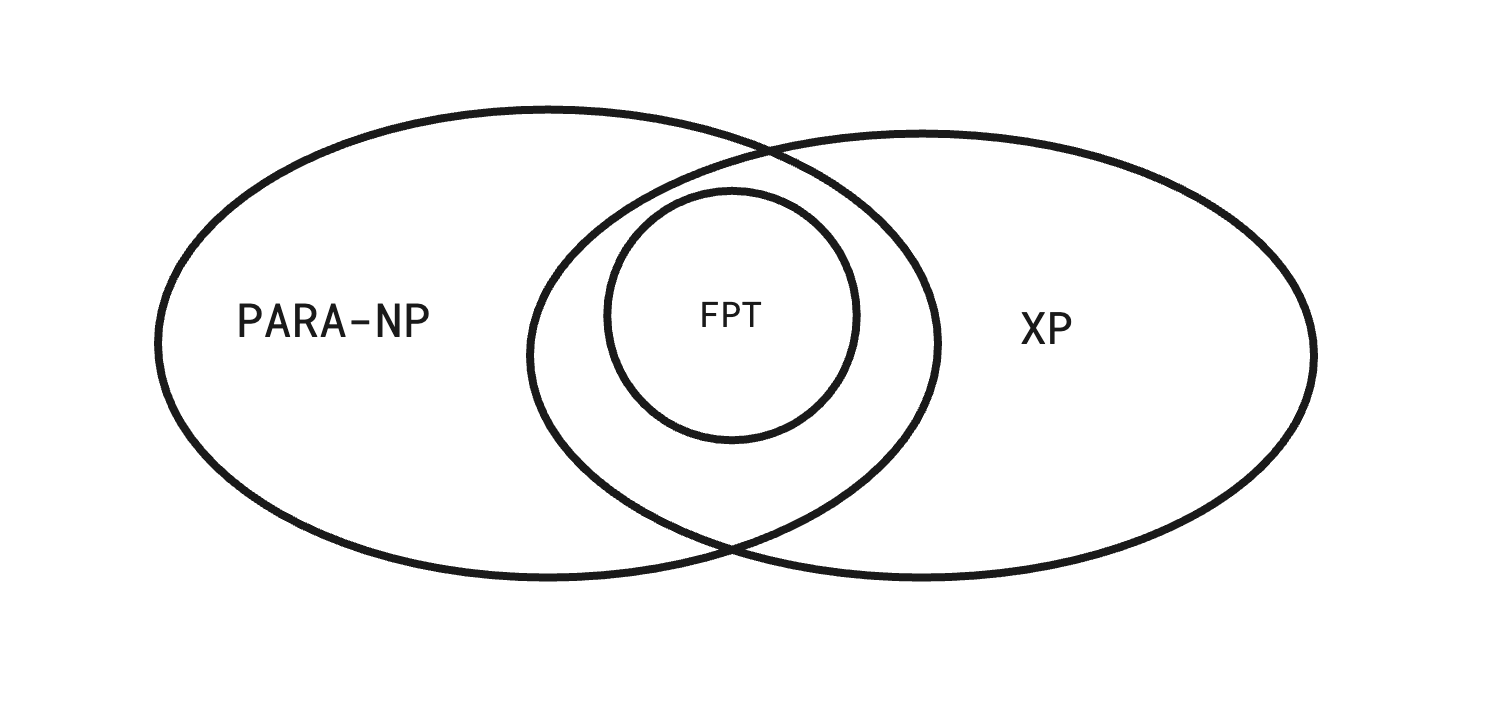
\includegraphics[width=0.8\linewidth]{img/para_comp}
	\caption{relazione tra le classi di complessità para-NP, XP, FPT}
	\label{fig:8}
\end{figure}

\subsection{Classe XP}
La classe XP rappresenta quei problemi parametrizzati che possono essere risolti in tempo $n^{f(k)}$ per una qualche funzione $f$.

\subsection{Classe para-NP}
I problemi in questa classe vengono risolti da \textbf{algoritmi non deterministici} che eseguono in tempo pari a $t = f(k) \cdot {\vert x \vert}^{\bigcirc(1)}$ per una qualche funzione $f$ e per un parametro $k$ del problema; sappiamo che FTP = para-NP sse P = NP.

\subsection{Klam value}
Il klam value è il massimo numero di passi di computazione eseguibili dato un tempo di esecuzione limitato, è utilizzato per confrontare algoritmi FTP.

klam value: un valore $k$ massimo, per un problema, t.c. risolve il problema con un vincolo di tempo $x$ (tipicamente $x$ assume il valore $10^{20}$ passi di computazione).

Ricordiamo che la funzione di complessità temporale relativa agli algoritmi FTP è del tipo $f(k) \cdot n^c$, quindi possiamo anche limitare $c$ con un valore $\leq3$, questo viene fatto per evitare di spostare tutta la complessità computazionale in questa parte della funzione che vincola il tempo

Prendiamo ora in considerazione la funzione per VC: se poniamo $k^2 \cdot 1,3^{20} = 10^{20}$ si ottiene un $k \sim 130$.

Se fossimo in grado di manipolare l'algoritmo e passare da $1,3 \rightarrow 1,2$ allora k cambierebbe nella seguente maniera: $k^2 \cdot 1,2^{20} = 10^{20}$ si ottiene un $k \sim 190$, quindi, avendo due algoritmi, quello con il klam value maggiore può essere utilizzato con uno spettro maggiore di parametri.

\section{k-VC}
k-VC è la versione di decisione di VC; richiede di trovare, se esiste, una copertura del grafo, tale che il numero di vertici che sono nella copertura sia $\leq$ k; più formalmente: dato un grafo $G = \langle V, E\rangle$, richiede di trovare una copertura $V'$ ossia: $$ V'\subseteq V \quad \vert \quad \vert V' \vert \leq k \wedge \forall (u, v) \in E \Rightarrow (u \in V' \vee v \in V') $$
k-VC è un problema FPT, esiste infatti un algoritmo che esegue in tempo $2^k n^{\bigcirc(1)}$; un algoritmo per risolvere k-VC è chiamato "bounded search tree", l'idea è la seguente: si sceglie ripetutamente un vertice, quindi si effettua una scelta: aggiungere lui oppure tutti i suoi vicini alla cover.

\subsection{Kernelization for k-VC}
In generale, la kernelizzazione è una tecnica con la quale si prende l'istanza di un problema e si cerca di diminuirne la dimensione, ottenendo così un kernel, ciò viene ottenuto tramite una fase di preprocessing; la kernelizzazione è utile in quanto risolvere il problema dato sul kernel è al massimo difficile tanto quanto risolvere il problema sull'istanza originale; la kernelizzazione viene spesso realizzata tramite un insieme di regole di riduzione che rimuovono parti dell'istanza che sono facili da gestire. Vediamo ora un esempio di kernelizzazione per k-VC sul grafo $G = (V, E)$ considerando al massimo $k$ vertici:
\begin{enumerate}
\item Se $k > 0$ e $v \in V \mid degree(v) > k$ allora si deve rimuovere $v$ da $V$, quindi $k--$ (è necessario aggiungere il vertice $v$ in quanto, altrimenti bisognerebbe includere tutti i sui vicini nella copertura, ciò significherebbe sforare il limite del parametro $k$, questo è valido per tutti i vertici con grado maggiore di $k$).
\item Rimuovere da $G$ tutti i vertici $v$ isolati (che non hanno archi entranti / uscenti).
\item Se rimangono \textbf{più} di $k^2$ archi, e, sia la regola 1 che la regola 2 non possono più essere applicate, allora il grafo non ha una cover di dimensione $\leq k$, in quanto significa che si potranno prendere al massimo $k$ vertici, ma ognuno di essi avrà al massimo grado $k$ (per la regola 1) e quindi potendo prendere al massimo $k$ vertici che hanno al massimo grado $k$, si potranno coprire al massimo $k^2$ archi, non si sarebbe quindi in grado di soddisfare i vincoli.
\end{enumerate}

\section{K-Independent Set}

\section{K-clique}
L'input di questo problema è il seguente: un grafo $G = (V, E)$, un parametro $k$, l'output sarà quindi un clique di $k$ vertici (se esiste)

\pagebreak
\part{SAT solvers}

\section{Problema - SAT}
Satisfiability (SAT) è il seguente problema: data un formula booleana in CNF, è possibile soddisfarla oppure no?

\subsection{3-SAT}
3-SAT è simile a SAT, solo che si pone un vincolo alla dimensione di ogni clausola: ogni clausola avrà al massimo tre letterali. Sappiamo che 3-SAT appartiene ai para-NP; idea della dimostrazione: siccome un algoritmo A FPT per 3-sat sarebbe $A = T(n, k) = 2^n \cdot n^{\bigcirc(1)} = 2^3 \cdot n^\alpha$ questo significherebbe trovare un algoritmo polinomiale in $n$ per 3-SAT, ma sappiamo essere falso a meno che $P = NP$.

\subsection{SAT-n}
SAT-n è SAT con un numero n di letterali, si dimostra che $SAT-n \in FPT$, infatti $T = \bigcirc(2^n \cdot m)$ con n = numero di letterali, m = dimensione dell'input. In questo caso si può notare che abbiamo $m^1$ quindi questo caso specifico non è solo FPT, ma appartiene ad una classe più ristretta: FPL(ossia Fixed Parameter Linear).

\subsection{Approccio - SAT solvers}
Un SAT solver ritorna se un'istanza del problema SAT $\in$ SAT oppure $\notin$ SAT. Analizziamo i SAT solver anche se non sono sui grafi in quanto:
\begin{itemize}
\item SAT è NP-comp/NP-hard.
\item SAT è uno dei problemi più studiati, quindi sono stati sviluppati diversi tools per cercare di risolverlo.
\item Siamo in grado di mettere in relazione SAT con un problema sui grafi.
\end{itemize}
Vediamo ora alcuni SAT solver:
\begin{itemize}
\item DPLL: tutti i migliori algoritmi sono basati su questo, quindi, ogni algoritmo specifico migliora un determinato aspetto, per sfruttare le proprietà della formula SAT data; bisogna comunque ricordare che non esiste un SAT solver migliore di tutti gli altri, dipende dalla formula.
\item Solver in parallelo:
\begin{itemize}
\item Portfolios: il funzionamento dei portfolios è quello di eseguire in parallelo diversi algoritmi su una stessa istanza, oppure uno stesso algoritmo ma con diverse configurazioni, su una stessa istanza; questo è utile in quanto non si può sapere a priori quale solver sia più efficente data un'istanza di SAT.
\item Divide and conquer: i SAT solver di questo tipo cercano di dividere lo spazio di ricerca così da poter assegnare ogni spazio identificato ad una data risorsa (processore), così da rendere più rapida la ricerca di una soluzione.
\end{itemize}
\end{itemize}

\subsubsection{Approccio - DP solver}
Vediamo ora come funzione il SAT solver più famoso, ossia DP: Davis-Putnam.

DP è composto da tre regole:
\begin{enumerate}
\item \textbf{Unit-propagation}: se noto che esiste una clausola con un solo letterale, ad esempio: $$ \phi = (x_1 \vee x_3) \wedge (x_2 \vee x_4) \wedge (x_2)$$ nella formula sopra notiamo che l'ultima clausola è formata da un solo letterale, quindi possiamo affermare che $\phi$ è soddisfatta sse $$\phi' = \phi \wedge (x_2 = 1)$$ è soddisfatta.

Ora possiamo quindi rimuovere tutte le occorrenze di $x_2$ e $\overline{x_2}$.

Quindi la formula diventerà $\phi' = (x_1 \vee x_3) \wedge (x_4) \wedge (x_2 = 1)$.

Si noti che ora la regola può essere riapplicata alla clausola $(x_4)$; quindi, l'algoritmo DP tipicamente esegue questa regola fino a che non è più possibile, per semplificare di molto la formula data.
\item \textbf{Pure literal}: se noto che un letterale appare solo in forma positiva o negativa (può apparire anche più volte): $$ \phi = (x_1 \vee \overline{x_2} \vee x_3) \wedge (\overline{x_1} \vee \overline{x_4} \vee \overline{x_3}) \wedge (\overline{x_2} \vee x_4 \vee \overline{x_1})$$
nella formula sopra notiamo che $x_2$ appare solo in forma negata, quindi posso sfruttare questa proprietà per semplificare tutte le clausole che contengono $\overline{x_2}$, in quanto, settando $x_2 = 0$ avrò $\overline{x_2} = 1$, ottenendo quindi $$\phi' = (\overline{x_1} \vee \overline{x_4} \vee \overline{x_3}) \wedge (\overline{x_2} = 1)$$
Anche questa regola, come la unit propagation, viene tipicamente applicata il più possibile, per fare in modo di semplificare di molto la formula.
\item \textbf{Resolution rule}: la resolution rule consiste nell'assegnare un valore di verità ad un letterale, sollevando così due questioni:
\begin{enumerate}
\item Come scelgo il letterale su cui effettuare l'assegnamento? questo è un punto che influenza molto il tempo di esecuzione, infatti la scelta di un letterale più adeguato porta ad una maggior efficienza dell'algoritmo; facciamo quindi alcune considerazioni:
\begin{itemize}
\item Scelta random? non ha senso potremmo prendere il "peggiore".
\item Scegliere un letterale che appaia in maniera bilanciata (tanti valori negativi quanti positivi).
\item Scegliere un letterale che appaia molte volte.
\item Scegliere un letterale che appare in clausole con esattamente due letterali, questo significa che, una volta effettuata la scelta, si potrà applicare la unit propagation.
\end{itemize}
\item Assegno 0 o 1 al letterale scelto? assegnare 0 piuttosto che 1 al letterale scelto porta ad un risultato escludendone un altro, ci si potrà rendere conto più avanti nell'esecuzione se la scelta è stata buona oppure no, infatti, alcune scelte (es $x_1 = 0$) potrebbero rendere la formula impossibile da soddisfare, richiedendo quindi di effettuare backtracking per effettuare la scelta opposta (es $x_1 = 1$); il tipo di backtracking visto da noi vuole che si effettui backtracking sull'ultima scelta effettuata: considerando la figura \ref{fig:9}, è stata precendentemente applicata la resolution rule sulle variabili $a = 0$, $b = 0$, $c = 0$, quindi, siccome la scelta di $c = 0$ porta ad un conflitto, si effettua backtracking all'ultima variabile su cui è stata applicata la resolution rule ($c$) e si cambia il valore dell'assegnamento; verrà quindi posto $c = 1$.
\begin{figure}[h]
	\centering
	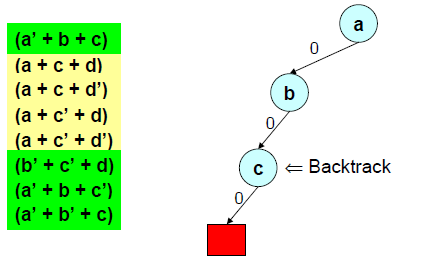
\includegraphics[width=0.8\linewidth]{img/Dpll_backtrack.png}
	\caption{Esempio di backtracking su algoritmo DPLL}
	\label{fig:9}
\end{figure}
\end{enumerate}
\end{enumerate}

\subsubsection{Conflict Driven Clause Learning - CDCL}
CDCL è un altro SAT solver, basato su DDPL, vi sono due differenze principali tra i due:
\begin{itemize}
\item CDCL utilizza un implication graph per migliorare la qualità delle scelte, infatti è proprio questo grafo che permette di effettuare backjumping al posto di backtracking.
\item CDCL effettua backjumping (backtracking non-cronologico) a differenza di DPLL che effettua backtracking, questo permette di risparmiare molto tempo saltando direttamente alla scelta del letterale che causa un conflitto.
\end{itemize}

\subsection{Riduzione da VC a SAT}
Vediamo una riduzione polinomiale da VC a SAT:
\begin{itemize}
\item I vertici di VC corrispondono alle variabili di SAT.
\item La clausola $(x_i \vee x_j)$ esiste sse $(v_i, v_j) \in E$.
\end{itemize}

\pagebreak
\part{Tour problems}

\section{Problema - Hamiltonian path}
Il problema Hamiltonian path (HP) è il seguente:
\begin{itemize}
\item Input: $G = (V, E)$
\item Output: esiste un path che visita tutti i vertici 1 ed 1 sola volta?
\end{itemize}
nota: HP $\in$ NP-comp.

\subsection{Hamiltonian Cycle}
Hamiltonian cycle è simile a Hamiltonian path, ad eccezione che si richiede di trovare un ciclo che tocca tutti i vertici una ed una sola volta, invece di un path; un Hamiltonian path che inizia e finisce in due vertici adiacenti può essere trasformato in un Hamiltonian cycle aggiungendo l'arco che collega i due e viceversa (da HC a HP).

HC è considerato un caso particolare del problema TSP, dove, a partire da un'istanza di TSP, si cambia il peso degli archi: la distanza tra due città viene posta pari a 1 se sono adiacenti, a 2 se non sono adiacenti, quindi, si verifica se la distanza percorsa è pari a $\vert V \vert$, quindi, se lo è, il path è un HC.

\subsection{Approcci per Hamiltonian Path}
Analizziamo ora alcuni approcci possibili per HP:

\begin{itemize}
\item Brute force (non va bene, esponenziale n!).
\item Possibilità di classificare gli archi (più o meno) come si è fatto in Eulerian Path con i vertici, quindi dividerli in:
\begin{itemize}
\item Archi da usare.
\item Archi da non usare.
\item Decidere arbitrariamente se usare o no un determinato arco.
\end{itemize}
\item Programmazione dinamica, un esempio può essere questo: $(S, v)$ con S set di vertici e v vertice finale, quindi possiamo trasformarlo in $(S_{\setminus \lbrace w \rbrace}, w) \wedge (w, v) \in E$; notiamo però che anche questo approccio richiede tempo esponenziale: $\bigcirc(n^2 \cdot 2^n)$.
\item Siccome SAT appartiene a NP-comp, allora possiamo applicare i SAT-solver per risolvere HP
\item Utilizzando un approccio non convenzionale: DNA computing.
\end{itemize}

\section{Problema - Eulerian path}
Il problema è così formulato:
\begin{itemize}
\item Input: grafo $G=(V, E)$.
\item Output: esiste un path di G che attraversi, una ed una sola volta, tutti gli archi di E? (nota: permette di passare più volte da uno stesso vertice).
\end{itemize}
possiamo notare che un Eulerian path esiste sse una delle due situazione è verificata:
\begin{itemize}
\item Si hanno solo nodi con grado pari.
\item Si hanno esattamente due nodi con grado dispari, quindi uno dei due sarà quello di partenza e l'altro quello di arrivo.
\end{itemize}
Possiamo quindi affermare che controllare se esiste un EP equivale a controllare se una delle due proprietà enunciate è rispettata, ed è quindi possibile verificare se esiste un EP in tempo polinomiale rispetto all'input, in quanto il controllo delle due proprietà richiede una visita di tutti i vertici.

\textbf{Nota}: il grado di un vertice indica il numero di archi incidenti in esso; (quindi nel caso di un grafo orientato, indica il numero di archi con origine in esso, che è anche visto come il numero di figli).

\section{Problema - TSP}
Il problema TSP (Travelling Salesman Problem) è così formulato:

Input:
\begin{itemize}
\item Un grafo $G = (V, E)$ completo e simmetrico (il peso di un arco è uguale nelle due direzioni).
\item Una funzione $W: E \rightarrow R^+$ indica il peso di ogni arco.
\end{itemize}
Output: qual'è il minimo HP (Hamiltonian Path)? Si noti che non si dovrà controllare se esista l'HP, in quanto abbiamo detto che G è completo, quindi sicuramente almeno un HP esiste.

\subsection{Approccio - Algorithms for TSP}
Analizziamo ora alcuni approcci possibili per TSP:
\begin{itemize}
\item Brute force (non va bene per il tempo esponenziale).
\item Dynamic programming; ma ha sempre un tempo esponenziale.
\item Nearest neighbour: è un algoritmo che in molti casi performa molto bene, ma vi sono alcuni casi in cui invece performa molto male, quindi può essere interessante; (c'è un problema, ossia che mano a mano che si effettuano delle scelte, ci si preclude la possibilità di effettuarne altre che potrebbero essere migliori).
\item Algoritmi approssimanti? per TSP non esistono a meno che P = NP:
\end{itemize}

\subsection{Problema TSP-decisione}
Il problema TSP-d, una variante di TSP, è così formulato:

Input:
\begin{itemize}
\item Un grafo $G = (V, E)$ completo e simmetrico (il peso di un arco è uguale nelle due direzioni).
\item Una funzione $W: E \rightarrow R^+$ indica il peso di ogni arco.
\item Un parametro d che indica un peso.
\end{itemize}
Output: Esiste un HP (Hamiltonian Path) t.c. $w(hp) \leq d$? Si noti che, anche in questo caso, non è necessario controllare se esista l'HP, in quanto abbiamo detto che G è completo, quindi sicuramente almeno un HP esiste.

\subsection{Problema TSP-metrico}
Il problema TSP-metrico, una variante di TSP, è così formulato:

Input:
\begin{itemize}
\item Un grafo $G = (V, E)$ completo e simmetrico (il peso di un arco è uguale nelle due direzioni).
\item Una funzione $W: E \rightarrow R^+$ indica il peso di ogni arco.
\item G soddisfa la disuguaglianza triangolare, ossia che per ogni coppia di archi t.c.:  $(a, b)$ $(b, c) \in E$, allora possiamo affermare che $w(a, b) + w(b, c) \geqslant w(a, c)$
\end{itemize}
Output: qual'è il minimo HP (Hamiltonian Path)?

Si noti che non si dovrà controllare se esista l'HP, in quanto abbiamo detto che G è completo, quindi sicuramente almeno un HP esiste.

\subsubsection{Approcci per TSP metrico}
Analizziamo ora alcuni approcci possibili per TSP metrico:
\begin{itemize}
\item Nearest neighbour per TSP-metrico è tipicamente molto buono, ed ha un fattore di approssimazione uguale a $\Theta(log \vert n \vert )$.
\end{itemize}

\subsubsection{TSP metrico - 2-opt}
Un algoritmo 2-opt per TSP metrico è il seguente:
\begin{itemize}
\item Si costruisce il MST (chiamato T) del grafo originale.
\item Si effettua una DFS traversal (chiamato D) di T.
\item Si prende D e si rimuovono tutti i vertici che vengono attraversati più di una volta (possiamo bypassare i vertici doppi in quanto sappiamo che il grafo è completo), ottenendo cosi un tour che è al massimo il doppio del tour ottimo, infatti, considerando figura \ref{fig:10} possiamo notare come il percorso, che parte dal vertice $a$, in verde passi esattamente due volte da ogni arco, e siccome noi invece abbiamo al massimo tanti archi quanto il MST, allora possiamo affermare che $W_{tour} \leq 2 * opt$.
\end{itemize}

\subsubsection{TSP metrico - Christofides}
L'algoritmo di Christofides migliora il risultato dell'algoritmo 2-opt precedente, utilizzando minimum-weight perfect matching, ottenendo così un algoritmo 1,5-opt: $W_{tour} \leq 1.5 * opt$. I passi dell'algoritmo sono i seguenti:
\begin{itemize}
\item Si costruisce il MST (chiamato T) del grafo originale.
\item Si costruisce un insieme S a partire da T contenente tutti i vertici con grado dispari.
\item Si esegue un algoritmo min-cost-perf-matching sull'insieme S ottenendo dei nuovi archi E'.
\item Aggiungiamo gli archi E' a T (facendo così in modo che tutti i vertici in T abbiano grado pari).
\item Cercare un Eulerian path in T.
\item Bypassare tutti i vertici che si ripetono.

\end{itemize}

\begin{figure}[h]
	\centering
	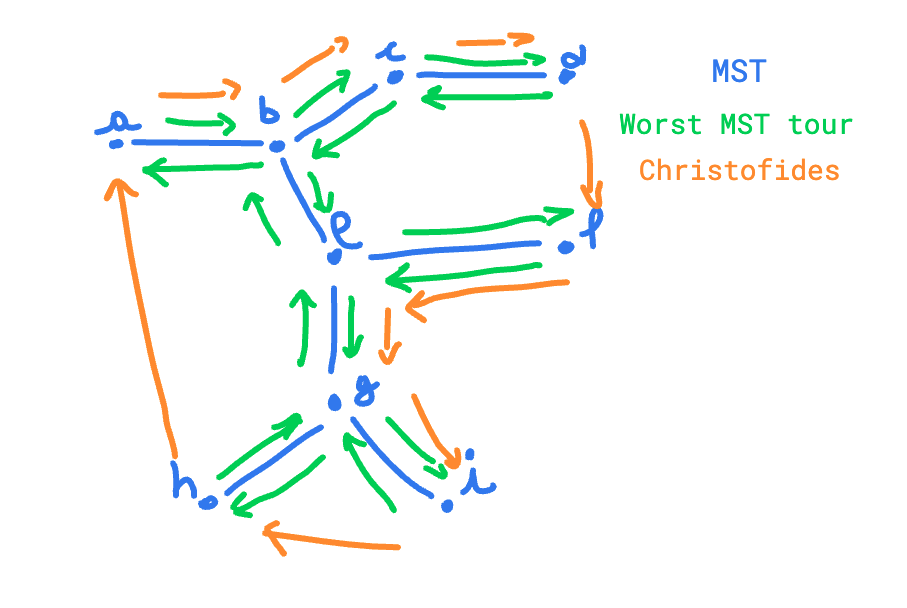
\includegraphics[width=1\linewidth]{img/Christofides}
	\caption{MST di un grafo}
	\label{fig:10}
\end{figure}

\subsubsection{Approccio - TSP metrico - K-opt - Lin-Kernighan}
Un'altra miglioria che si può apportare ad un  tour è quella di applicare k-opt, l'idea principale di questi algoritmi è di prendere una sezione di path che ha un x crossing, quindi riordinarla in maniera tale che ciò non avvenga;analizziamo ad esempio 2-opt, consideriamo la figura \ref{fig:11}, notiamo come "x crossing" venga risolto, questo può portare ad una miglioria nel tour, $T(2-opt) = \bigcirc(n^2)$; 3-opt farà una cosa simile, ma considerando 3 archi invece che 2, 3-opt richiede anche più tempo rispetto a 2-opt $T(3-opt) = \bigcirc(n^3)$, ma a favore di possibili risultati migliori rispetto a 2-opt.
\begin{figure}[h]
	\centering
	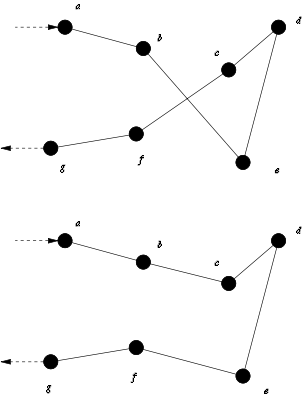
\includegraphics[width=0.5\linewidth]{img/2-opt_wiki.svg.png}
	\caption{Effetto dell'algoritmo 2-opt}
	\label{fig:11}
\end{figure}
Considerando quindi k-opt, l'idea di Lin-Kernigham è di partire applicando il k minore (2) e via via aumentare k, questo non significha che se arriviamo a k=4 allora tutti i calcoli precedenti sono stati inutili, infatti l'elaborazione di k=2 può aver "aiutato" k=3 ecc. Per quanto riguarda TSP, se consideriamo il caso in cui non fosse simmetrico, si può comunque applicare 2-OPT, però considerando entrambi i versi, quindi, la condizione che deve essere rispettata è che:$$d(x_1, y_1) + d(x_2, y_2) \leq d(x_1, x_2) + d(y_1, y_2))$$
Generalmente si può ottenere 3-OPT a partire da 2-OPT complicandone alcune mosse; tipicamente Lin-Kern parte da 2-OPT, continua ad aumentare il K, fino a che non si migliora più.

\pagebreak
\part{Linear programming approach for TSP}

\section{Formulazione ILP - TSP}
Vedremo due formulazioni ILP di TSP, entrambe condividono le seguenti variabili:
\begin{itemize}
\item Le città vengono etichettate con numeri da $1,...,n$.
\item Il costo da una città ad un altra è sempre maggiore di zero: $c_{ij} > 0$.
\end{itemize}
La variabile principale del problema è $x_{ij}$ che assume i seguenti valori:
\begin{itemize}
\item $1$ se il path va dalla città $i$ alla città $j$.
\item $0$ altrimenti.
\item Nota: è a causa di questa variabile che la formulazione diventa non solo LP, ma ILP, infatti tutte le altre variabili sono lineari.
\end{itemize}
La funzione obiettivo è quindi la seguente (minimizzare lunghezza del tour):$$ min \displaystyle\sum_{i = 1}^{n} \sum_{j \neq i, j = 1}^{n} {c_{i j} \cdot x_{i j}}$$
Non è però abbastanza, è infatti necessario includere anche i due seguenti vincoli per fare in modo che ogni vertice abbia esattamente un solo arco entrante ed uno uscente:
$$ \displaystyle\sum_{i = 1, i \neq j}^{n} {x_{i j} = 1 \quad \forall j \in \lbrace 1,...,n \rbrace }$$
$$ \displaystyle\sum_{j = 1, j \neq i}^{n} {x_{i j} = 1 \quad \forall i \in \lbrace 1,...,n \rbrace }$$

\subsection{Formulazione - ILP - DFJ}
La particolarità di DFJ è la subtour elimination constraint: $$\displaystyle\sum_{i \in Q} \sum_{i \neq j, j \in Q} {x_{ij} \leq \vert Q \vert - 1} \quad \forall Q \subsetneq \lbrace 1,...,n \rbrace , \vert Q \vert \geq 2$$
La subtour elimination contraints implica che non vi sia un sottoinsieme di $Q$ che può essere un subtour di $Q$, quindi la soluzione ritornata sarà un singolo tour e non l'unione di più tour "piccoli".

\subsection{Formulazione - ILP - MTZ}
In questa formulazione vi è anche un'altra variabile: $u_i$, che tiene traccia dell'ordine in cui vengono attraversate le città, gestita nella seguente maniera: $$u_j + (n - 2) \geq u_i + (n - 1) \cdot x_{ij}$$
Si noti che le parti $(n - 2)$ e $(n - 1)$ sono inserite per gestire il caso in cui $x_{ij}$; si necessita anche del seguente vincolo: $$2 \leq i \leq n$$ ciò implica che sia un singolo tour a coprire tutte le città, e blocca la possibilità che siano uno o più tour disgiunti che, solo collettivamente, coprono tutte le città.

\subsection{Formulazione MILP - TSP}
Un'altra possibile formulazione per TSP è MILP, ossia Mixed Integer Linear Programming, a differenza di ILP, MILP permette di avere un rilassamento su alcune variabili, ossia permette di avere variabili che appartengono all'intervallo $[0, 1]$ al posto che appartenere all'insieme $ \lbrace 0, 1 \rbrace $.

\subsection{Politopo}
Un politopo è una rappresentazione dello spazio delle possibili soluzioni di un problema dato, considerando la figura \ref{fig:polyt}, essa rappresenta il problema matching sul grafo dato, sappiamo quindi che, siccome è un grafo completo, e contiene solo tre vertici, allora si potrà prendere al massimo un vertice per ottenere un matching, questo significa, che tra tutte le possibili soluzioni elencate nella tabella, si possono escludere tutte quelle che contengono più di un vertice, così riducendo lo spazio di ricerca.

\subsubsection{TSP Polytope}
Vogliamo ora definire un politopo specifico per il problema TSP, quindi, considerando la formulazione ILP del problema, essa ha una variabile $x_{i, j}$ che è pari a $1$ se l'arco da $i$ a $j$ viene incluso nella soluzione, $x_{i, j} = 0$ altrimenti, allora il politopo per TSP sarà il seguente vettore: $TSP(n) = \lbrace x \in \lbrace0, 1\rbrace^{\vert E \vert}  \vert $ siano soddisfatti anche gli altri vincoli della formulazione $\rbrace $; si noti che il vettore descritto è di lunghezza $\vert E \vert$, quindi, dirà, per ogni arco del grafo, se esso appartiene alla soluzione oppure no, esattamente come la variabile $x_{i, j}$.

\begin{figure}[h]
	\centering
	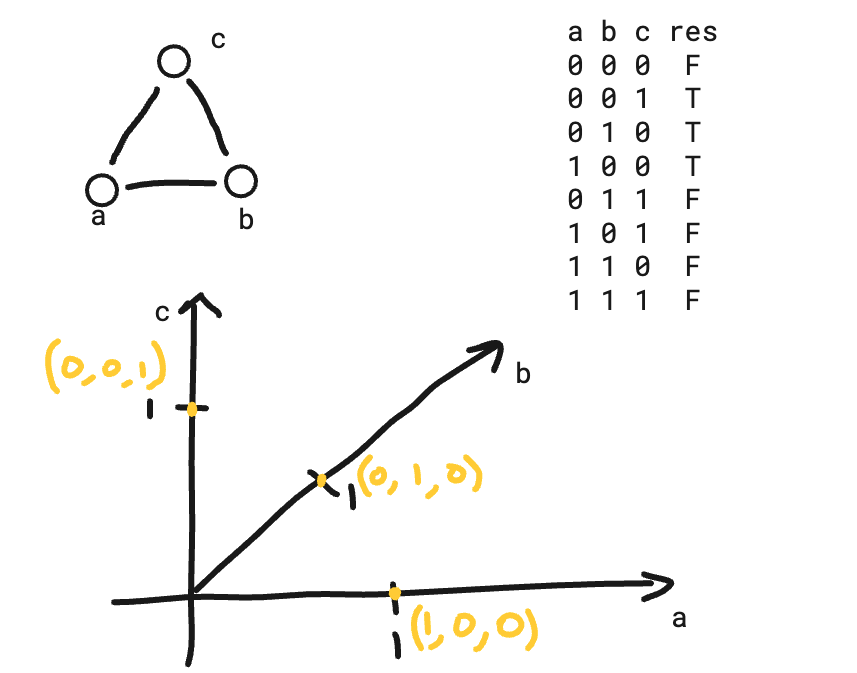
\includegraphics[width=0.8\linewidth]{img/polyt}
	\caption{Rappresentazione grafica del politopo relativo all'istanza precedentemente descritta del problema matching.}
	\label{fig:polyt}
\end{figure}

\subsection{Approccio - Simplesso}
Il simplesso è un metodo utilizzato per risolvere problemi espressi in formulazione linear programming. Nello specifico, considera il politopo relativo ad una determinata istanza, quindi si sposta da un vertice, che si trova sulla soglia tra regione ammissibile e non, all'altro, per cercare di migliorare il valore della funzione obiettivo; ricordiamo che la ricerca è effettuata sul confine perché è dimostrabile che la soluzione ottima si trova proprio in uno di quei punti.

\subsection{Rilassamenti}
Una tecnica che a volte funziona, per abbassare i tempi di esecuzione, è di rilassare alcuni vincoli del problema (nell'istanza di matching precedentemente presentata, un rilassamento potrebbe essere il seguente: al posto di avere al massimo 1 edge, ne ammetto 2).

Vediamo ora un rilassamento per il politopo per TSP descritto in precedenza: vogliamo considerare la possibilità di scegliere un arco solo parzialmente, per fare ciò dobbiamo permettere che le variabili $x_{i, j}$ non siano intere, bensì reali, il rilassamento che vogliamo sarà quindi: $TSP_R(n) = \lbrace x \in [0, 1]^{\vert E \vert}  \vert $ siano soddisfatti anche gli altri vincoli della formulazione $\rbrace $; un altro rilassamento potrebbe essere quello di "allargare" i restanti vincoli.

Si noti che una volta trovata una soluzione dopo aver applicato un rilassamento, ciò non significa che si termini, in quanto la soluzione che si ottiene tramite un rilassamento tipicamente è molto "basilare", l'idea è quindi di applicare un rilassamento, per ottenere una soluzione iniziale, quindi, a partire dalla soluzione ottenuta, cercare di migliorarla verso un ottimo locale.

\subsection{Approccio - Gomory's Cut}
Questo metodo richiede, come prima cosa, di rilassare il vincolo di interezza su $x_{i} \in \mathbb{N}$, facendolo passare a $x_{i} \in \mathbb{R}$, quindi si risolve il problema associato, ottenendo una soluzione "basica" (ossia un vertice); quindi, se il vertice (v) ottenuto come soluzione non è intero, allora questo metodo trova un hyperpiano con il vertice  (v) da un lato, e tutte le restanti feaseble solutions dall'altro, quindi l'hyperpiano dato viene aggiunto come vincolo lineare per escludere il vertice v, quindi si risolve il problema appena definito; si ripete questo procedimento fino a che il nuovo vertice trovato non è intero.

L'idea che sta dietro al trovare l'hyperpiano, di una soluzione, è di separare la parte intera dalla parte non intera di essa, vediamo un esempio:
$$ 3,2x_{1} +  1,5x_{2} - 2,3x_{3} = 2,5 $$
equivale a
$$ (3x_{1} +  1x_{2} - 2x_{3}) + (0,2x_{1} +  0,5x_{2} + 0,3x_{3}) = 2 + 0,5$$
il cutting plane sarà quindi:
$$ 0,2x_{1} +  0,5x_{2} + 0,3x_{3} \geq 0,5 $$
Nota: è un idea interessante, a volte funziona, altre volte no, non offre garanzie; infatti, nonostante l'idea di base sia quella di avvicinarsi sempre più ad un ottimo locale, a volte capita di tagliarlo fuori dallo spazio di ricerca, finendo quindi per allontanarsi da ciò che stavamo cercando.

\begin{figure}[h]
	\centering
	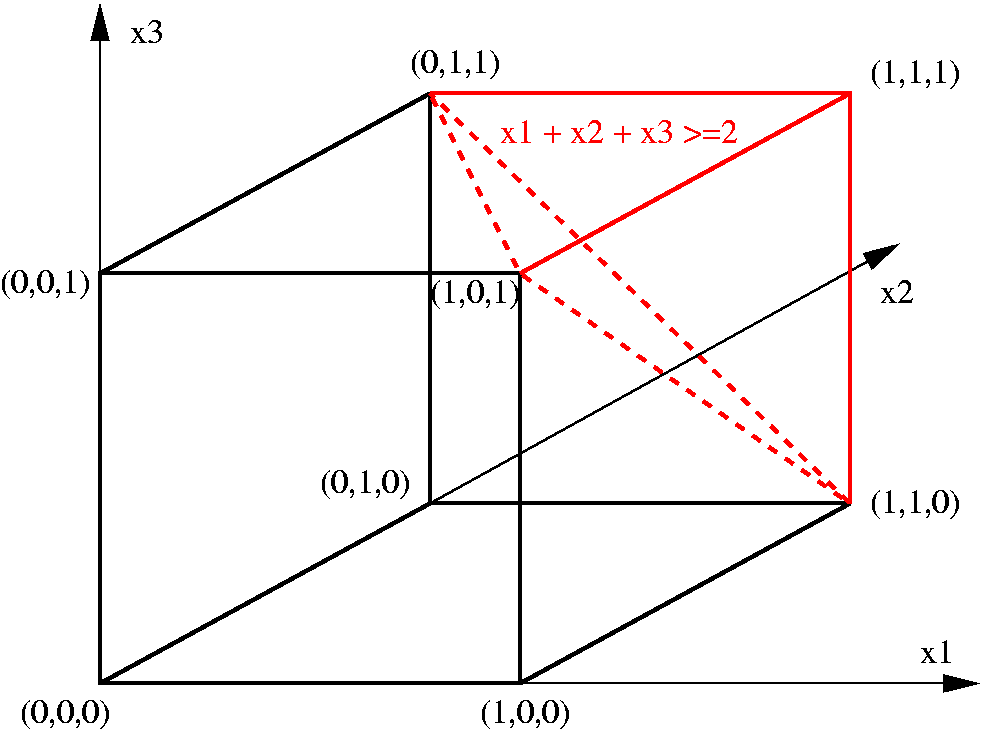
\includegraphics[width=0.8\linewidth]{img/TSP_cutting_plane.png}
	\caption{Rappresentazione grafica di un cutting plane per un istanza di TSP (il vincolo richiede che siano selezionati almeno due archi).}
	\label{fig:TSP_cutting_plane}
\end{figure}

\subsection{Approccio - Branch \& Bound}
Branch \& Bound è un metodo generale per risolvere problemi ILP; il funzionamento, come indica il nome, è il seguente:
\begin{itemize}
\item Branch part: separare il problema in due o più sotto problemi (spazi di ricerca), quindi, provare a risolvere separatamente ognuno di essi, ottenendo una soluzione per il problema principale.
\item Bound part: cercare di escludere parti del problema che non saranno utili, per risparmiare tempo di computazione.
\item È necessario sapere anche che tipicamente si tiene traccia di una best solution attuale, quindi di due bound (Upper bound: best solution raggiungibile teoricamente e Lower bound: best solution attuale).
\end{itemize}
Nota: la parte di bounding è necessaria in quanto, se non effettuata, allora si avrebbe sicuramente un algoritmo esponenziale, in quanto ogni nodo viene separato in più parti; ciò nonostante, effettuare la parte di bounding \textbf{non} garantisce che l'algoritmo trovi una soluzione in tempo polinomiale e, a volte è proprio la parte di bounding che allunga i tempi in quanto a volte servono molte iterazione per arrivare ad avere soluzioni intere.
Vediamo ora un algoritmo generico per Branch \& Bound:
\begin{enumerate}
\item $S = LB = 1$
\item $S^* = UP$
\item Branch $p$ as $p_1, p_2$ then $add(p_1, Q), add(p_2, Q)$
\item Take problem $p_i$ from $Q$ then $solve(p_i)$; $if(UB(p_i) \leq LB)$ then $prune(p_i)$
\item if $p_i$ is feaseble then
\begin{enumerate}
\item $B = bound(S_{p_{i}})$
\item if $B \geq LB$ then  $LB = B$
\end{enumerate}
\item else
\begin{enumerate}
\item Branch $p_i$ as $branch(p_{i, 1}, p_{i, 2})$ then $add(p_{i, 1}, Q), add(p_{i, 2}, Q)$
\end{enumerate}
\end{enumerate}
Nota: la condizione della riga riga $4$ è valida per problemi di massimizzazione, per problemi di minimizzazione diventerà $if(LB(p_i) \geq UB)$ then $prune(p_i)$; invece la $5.b$ cambierebbe nella seguente maniera: $B \leq LB$ then  $LB = B$.

Vediamo ora un esempio di Branch \& Bound:
$$ max \quad z = 100 x_1 + 150 x_2 $$
$$ 8000 x_1 + 4000 x_2 \leq 40000 $$
$$ 15 x_1 + 30 x_2 \leq 200 $$
$$ x_1, x_2 \geq 0 \quad x_1, x_2 \in \mathbb{N} $$
La prima cosa da fare p di rilassare il vincolo sull'interezza delle variabili, la formulazione diventa quindi:
$$ max \quad z = 100 x_1 + 150 x_2 $$
$$ 8000 x_1 + 4000 x_2 \leq 40000 $$
$$ 15 x_1 + 30 x_2 \leq 200 $$
$$ x_1, x_2 \geq 0 \quad x_1, x_2 \in \mathbb{R} $$
La soluzione che si ottiene dalla formulazione data è la seguente (un modo plausibile per ottenere $LB$ è di rimuovere dalle variabili la parte non intera):
$$ s_1: \quad x_1 = 2,22 \quad x_2 = 5,56 \quad UB = 1055,26 \quad LB = 950$$
Quindi si può continuare, ad esempio effettuando branch su una delle due variabili (un metodo per scegliere la variabile è di prendere quella con la parte intera maggiore, oppure scegliere quella con la parte non intera più vicina a $0,5$, ecc...) noi utilizzeremo il primo approccio, quindi effettuiamo branch sulla variabile $x_2$ arrivando nello stato di figura \ref{fig:b_b_1};
\begin{figure}[h]
	\centering
	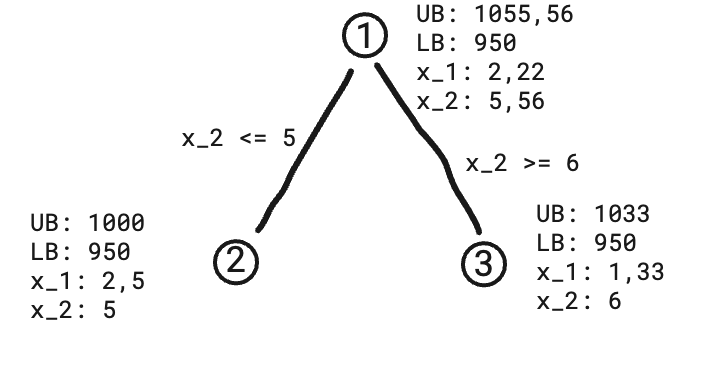
\includegraphics[width=0.8\linewidth]{img/b_b_1}
	\caption{}
	\label{fig:b_b_1}
\end{figure}
Quindi come scegliamo se andare avanti con il sotto problema $2$ oppure $3$? in questo caso si sceglie il sotto problema $3$ in quanto vogliamo massimizzare e $3$ ha un $UB$ maggiore di $2$; andiamo quindi avanti nell'esecuzione con il sotto problema $3$, facendo branch sulla variabile $x_1$; guardando figura \ref{fig:b_b_2} vediamo che il sotto problema $5$ non porta a nessuna soluzione; continuiamo quindi l'esecuzione con il sotto problema $4$ facendo di nuovo branch sulla variabile $x_2$, ottenendo figura \ref{fig:b_b_3} dove otteniamo una soluzione intera ($6$), abbiamo quindi un ultimo nodo da esplorare: $2$, ma notiamo che il suo $UB(2) \leq LB$ possiamo quindi potare $2$ ottenendo $6$ come soluzione finale, in quanto unica ed intera.
\begin{figure}[h]
	\centering
	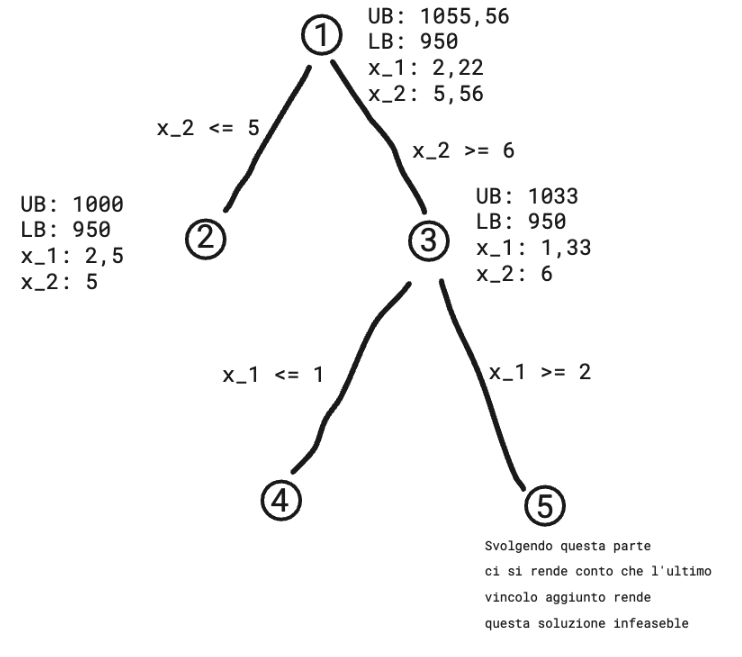
\includegraphics[width=0.8\linewidth]{img/b_b_2}
	\caption{}
	\label{fig:b_b_2}
\end{figure}
\begin{figure}[h]
	\centering
	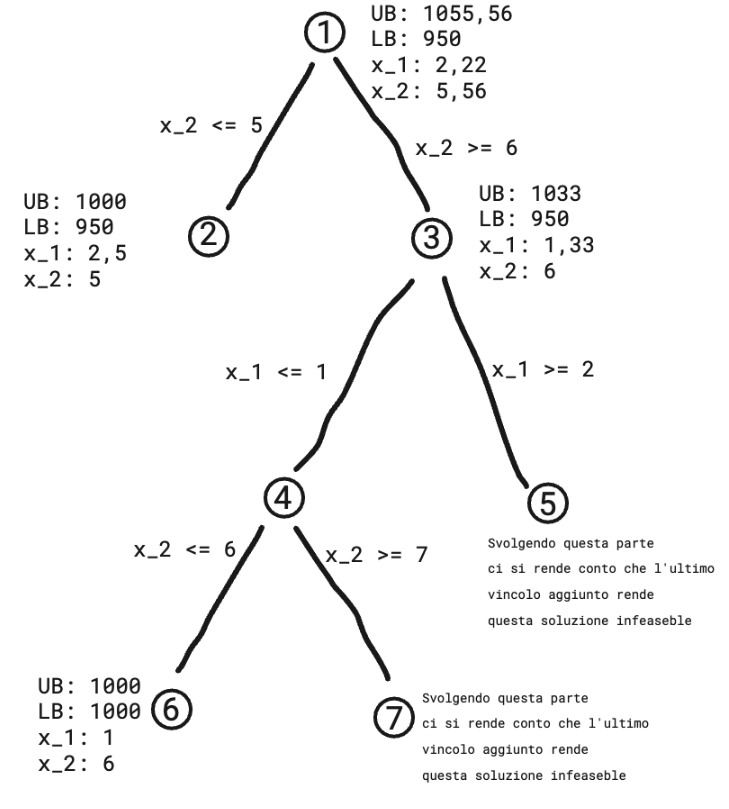
\includegraphics[width=0.8\linewidth]{img/b_b_3}
	\caption{}
	\label{fig:b_b_3}
\end{figure}

\subsection{Approccio - Branch \& Cut}
Questo metodo usa assieme i due metodi: Cutting planes e Branch \& Bound l'idea del metodo è la seguente: si applica B \& B, quindi si ottiene una soluzione non intera, allora si applica alla soluzione ottenuta un cutting plane, cercando di ottenere una soluzione intera in maniera rapida; un algoritmo generico per Branch \& Cut è il seguente:
\begin{enumerate}
\item $L, x^{*} = NULL$
\item $v^{*} = - \infty $
\item while (not-empty( $L$ ))
\begin{enumerate}
\item get-problem-from($L$)
\item solve($L_{relax}$)
\item if solve($L_{relax}$) is not feaseble, then go to $3$
\item else solve($L_{relax}$) = $x, v$, if $v \leq v^*$ then go to $3$
\item if $x$ is integer, then $x^* = x$, $v^* = v$ the go to $3$
\item else ($x$ is not integer) the add a cutting plane
\end{enumerate}
\end{enumerate}

\pagebreak
\part{Graph Drawing}

\section{Graph drawing}
Quando si disegna un grafo, vi sono alcune cose da tenere in considerazione:
\begin{itemize}
\item Mettere vicini tra loro i vertici connessi.
\item Evitare gli incroci tra archi.
\item Tipicamente le "foglie" vengono posizionate verso l'esterno.
\item Si vuole considerare la forma del disegno risultante.
\item Si vuole cercare di ottenere qualcosa di simmetrico, anche in questo caso migliorando la leggibilità.
\item Tipicamente viene usata sempre la stessa lunghezza per gli archi.
\item Tipicamente si usano linee dritte.
\end{itemize}
Si noti che l'elenco delle caratteristiche che abbiamo fatto sopra, non è necessariamente vero, infatti si potrebbero avere dei casi particolari in cui è preferibile modificare queste "best practices".

\subsection{Force-directed graph}
I forced-directed graph drawing sono una classe di algoritmi per disegnare grafi in maniera tale che siano più "belli", e quindi comprensibili da interpretare; alcune delle regole di questi algoritmi sono di cercare di usare la stessa lunghezza per tutti gli archi, di effettuare il minimo numero di incroci tra archi possibile. Questa classe di algoritmi è chiamata così in quanto simula effettivamente delle forze fisiche, per realizzare il disegno, tipicamente:
\begin{itemize}
\item La repulsione tra due vertici è effettuata dalla forza magnetica, tipicamente implementata tramite la legge di Coulomb: $F = k_e \dfrac{ \vert q_1 \vert \vert q_2 \vert }{d^2}$
\item L'attrazione tra due vertici è effettuata dalla forza di una molla, tipicamente implementata tramite la legge di Hooke: $F = k_c x $ dove x è la distanza tra due vertici.
\end{itemize}
Quando si utilizzano questi algoritmi, ci si potrà rendere conto che le formule utilizzate non daranno un risultato che consideriamo ottimale in termini di qualità del disegno, si può quindi andare a cambiare il modulo delle forze in gioco, ad esempio considerandole tramite un logaritmo, invece che considerarle in maniera "pura".

Analizziamo ora alcuni vantaggi e svantaggi della tecnica force-directed, seguono i vantaggi:
\begin{itemize}
\item Tipicamente si ottiene un buon risultato.
\item Flessibilità: a seconda dell'obiettivo che abbiamo, si può adattare l'algoritmo.
\item Semplicità: siccome l'algoritmo è semplice, se si ottiene un disegno molto sbagliato è possibile cambiare l'algoritmo per adeguare il risultato.
\item Interattività: con questi algoritmi vengono effettuati diverse iterazioni, quindi non si passa direttamente dal grafo originale a quello finale,è quindi possibile vedere i risultati delle iterazioni intermedie, per verificare se l'algoritmo sta funzionando correttamente.
\item Theoretical foundation: conosciamo ed utilizziamo da molto tempo (alcune anche secoli) le forze che vengono simulate in questi algoritmi, quindi abbiamo una certa dimestichezza e conoscenza di ciò che si sta manipolando.
\end{itemize}
Seguono gli svantaggi:
\begin{itemize}
\item Time complexity: durante l'esecuzione le forze vanno applicate ad ogni coppia di vertici, la complessità di un iterazione richiede quindi $\bigcirc({\vert V \vert}^2)$, considerato che, data l'esperienza, sappiamo che tipicamente si effettuano circa $\bigcirc(\vert V \vert)$ iterazioni per ottenere un buon risultato, allora il tempo totale è di $\bigcirc({\vert V \vert}^3)$
\item Poor minima: Anche in questo algoritmo, come in altri, si potrebbe incappare in un ottimo locale che limiterebbe molto il risultato finale.
\end{itemize}

\subsection{N-body simulation}
Anche questa tecnica (come la force-directed) serve per simulare leggi fisiche (e.g. gravità) che studiamo da molti anni, alcune anche da secoli, quindi abbiamo dimestichezza con i calcoli; in genere viene implementata tramite un sistema di equazioni da risolvere.

\subsubsection{Barnes–Hut simulation}
La Barnes–Hut simulation è un tipo di n-body simulation, lo scopo di questa tecnica è di abbassare i tempi di esecuzione; infatti, considerando quello che abbiamo detto nella sezione relativa all'approccio force-directed, si conclude affermando che richiede un tempo di esecuzione di circa $\bigcirc({\vert V \vert}^3)$, che è polinomiale, ma, per grafi di dimensioni molto grandi richiede comunque un tempo troppo elevato, quindi, visto che le forze repulsive, sono naturalmente locali, si può pensare di dividere il grafo in più partizioni, considerando quindi solo i vicini all'interno di una stessa partizione; Quindi, nel caso di una n-body simulation, per ogni partizione sarà necessario memorizzare solo la massa totale e il centro di massa. Questa fase verrà ripetuta più volte, fino a che, all'interno di una partizione, o vi è un solo vertice, oppure non vi sono vertici.

Questo approccio stile dividi et impera permette di diminuire il tempo di un iterazione, nello specifico, facendolo passare da $\bigcirc({\vert V \vert}^2)$ a $\bigcirc({\vert V \vert log(\vert V \vert)})$

\begin{figure}[h]
	\centering
	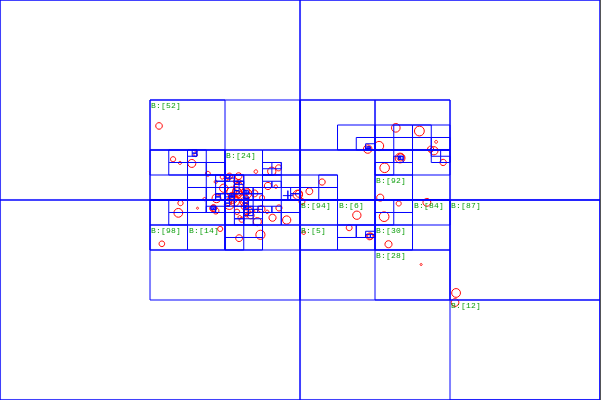
\includegraphics[width=0.8\linewidth]{img/2D_Quad-Tree_partitioning_of_100_bodies.png}
	\caption{Rappresentazione grafica di una 100-body simulation tramite Barnes–Hut}
	\label{fig:Barnes–Hut}
\end{figure}

\subsubsection{Barnes–Hut tree}
In questo caso vi è da fare una distinzione tra simulazione 3D e 2D, infatti, se si parla di 3D, allora l'algoritmo Barnes–Hut dividerà ricorsivamente il grafo in gruppi, memorizzando questi gruppi in un octree (oppure quadtree in 2D), quindi, ogni nodo sarà la rappresentazione di una partizione del grafo; il vertice radice rappresenta lo spazio per intero, quindi i suoi otto figli (quattro se si considera un quadtree), le foglie dell'albero, per quello che abbiamo detto in precedenza, o hanno 1 vertice oppure non ne hanno proprio.

\subsection{Gestione spazio disegno}
Quando viene effettuato il disegno della rappresentazione di un grafo, vogliamo che venga utilizzato all'incirca tutto lo sazio a disposizione, per fare in modo che la figura risulti più comprensibile; questo risultato è ottenibile utilizzando la tecnica vista fino ad ora (force-based) assieme ad una costante che consideri lo spazio a disposizione, ad esempio:
\begin{itemize}
\item La forza attrattiva avrà la generica forma: $f_a (d) = \dfrac{d^2}{k}$
\item La forza repulsiva avrà invece la generica forma: $f_r (d) = \dfrac{-k^2}{d}$
\item Dove la costante per gestire lo spazio a disposizione vale $k = c \sqrt{\dfrac{\textit{total area}}{\vert V \vert}}$
\item $c$ è un hyperparameter che permette di manipolare il risultato a piacimento, per ottenere il goal desiderato; tipicamente questi parametri assumono un valore all'interno di un determinato range.
\end{itemize}

\subsection{Particle Swarm Optimization - PSO}
Questa è un algoritmo sociale basato sugli stormi di uccelli che cercano cibo, da ciò deriva il nome. L'idea di questa tecnica applicata a graph drawing è che ogni particella non rappresenta un vertice, ma bensì una configurazione del grafo, ossia una possibile soluzione; Alcuni vantaggi di PSO sono i seguenti: 1) è altamente parallelizzabile 2) non usa il gradiente 3) utilizza pochi hyperparameters. Vediamo ora più nello specifico i parametri di un particella $P_i$, all'istante $t$:
$$P_i^{t} = [ x_{0, i}^{t}, x_{1, i}^{t}, x_{2, i}^{t}, ... ,x_{n, i}^{t},] $$
dove le varie $x_{i, j}^{t},$ sono le coordinate rispetto allo spazio, della particella i-esima all'istante di tempo $t$; si noti che è difficile trovare il giusto \textbf{equilibrio} tra numero di elementi e tempo di esecuzione, infatti, se si hanno troppi elementi, non solo si avrà un tempo di simulazione più alto del necessario, ma si incapperà nella situazione in cui si avranno alcune particelle sovrapposte (sulla stessa posizione) ed è quindi una situazione non ottimale. Oltre alle coordinate nello spazio, ad ogni particella è associata una velocità in un determinato istante di tempo $t$:
$$ V_{i}^{t} = [v_{0,i}^{t}, v_{1,i}^{t}, v_{2,i}^{t}, ... , v_{n,i}^{t}] $$
questa velocità indica il movimento della particella di riferimento in una data direzione; conoscendo quindi l'attuale posizione della particella ($P_i^{t}$) possiamo calcolare la successiva velocità: ($V_{i}^{t+1}$), quindi, una volta calcolata la velocità successiva, possiamo calcolare la posizione successiva della particella:
$$ P_{i}^{t+1} =  P_{i}^{t} + V_{i}^{t+1}$$
dove
$$V_{i}^{t+1} = w V_{i}^{t} + c_1 r_1(P_{PB, i}^{t} - P_{i}^{t}) + c_2 r_2 (P_{GB}^{t} - P_{i}^{t})$$
con:
\begin{itemize}
\item $w V_{i}^{t}$ parametro che serve come sorta di inerzia che permette di modificare la velocità solo in un certo range; questa scelta di implementazione rende l'algoritmo più simile al comportamento degli uccelli veri, infatti, un uccello che ha visto un pezzo di cibo nel punto $A$, e quindi inizia ad avvicinarsi ad esso, se dopo alcuni istanti di tempo si accorge che c'è un altro pezzo di cibo nel punto $B$, allora esso non cambierà direzione in un istante, ma ci metterà almeno qualche istante.
\item $c_1 r_1(P_{PB, i}^{t} - P_{i}^{t})$ questa è la personal knowledge, ossia ciò che conosce la particella.
\item $c_2 r_2 (P_{GB}^{t} - P_{i}^{t})$ questa è la global knowledge, ossia il pensiero comune del gruppo.
\end{itemize}
Facciamo ora delle considerazioni sui valori assunti dai parametri:
\begin{itemize}
\item $r_1 \in [0, 2]$ è ciò che pensa la particella, all'inizio assume un valore random.
\item $r_2 \in [0, 2]$ è ciò che pensa il gruppo, all'inizio assume un valore random.
\item $w$ tipicamente $\simeq 0,72$.
\item $c_1$ tipicamente $\simeq 2,05$ da notare che è un valore simile a $r_1$.
\item $c_2$ tipicamente $\simeq 2,05$ da notare che è un valore simile a $r_2$.
\item tipicamente si cerca di ottenere che $c_1 + c_2 \geq 4$.
\end{itemize}

\subsubsection{$c_1$ \& $c_2$ setup}
Ora possiamo discutere di un'altra opzione, ossia si può scegliere di tenere $c_1$ e $c_2$ statici, oppure si può scegliere di farli variare nel tempo; avere un valore più alto di $c_1$ rispetto a $c_2$ significa che si da valore al pensiero della particella e quindi si favorisce la fase di exploration, viceversa, si starà favorendo la fase di exploitation.

Quindi, un buon metodo per settare $c_1$ e $c_2$ è di iniziare con $c_1$ molto alto e $c_2$ molto basso, quindi, abbassare gradualmente $c_1$, e alzare gradualmente $c_2$, si noti che al termine non si dovrà avere $c_1 = 0$ e $c_2 = max$, altrimenti nessuno si avvicinerà più all'ottimo, è quindi importante che $c_1$ non sia mai pari a $0$.

\subsubsection{Quando fermarsi?}
L'algoritmo verrà arrestato se si è arrivati ad un tempo di esecuzione pari a circa $\vert V \vert$; nel caso specifico di graph drawing, una volta che la procedura è terminata, si deve scegliere la particella migliore, confrontando le varie particelle tra loro.

\subsubsection{Relazione tra PSO e graph drawing}
Quando vogliamo applicare PSO dobbiamo trovare un modo per mettere in relazione la descrizione di PSO con il problema graph drawing, ad esempio, considerando la seguente formula:
$$P_i^{t} = [ x_{0, i}^{t}, x_{1, i}^{t}, x_{2, i}^{t}, ... ,x_{n, i}^{t},] $$
avremo che ogni $x$ deve rappresentare uno specifico vertice, nello specifico, le coordinate di un vertice, si noti quindi che, a seconda della dimensionalità del disegno (2d, 3d, ecc...) ogni $x$ non sarà un singolo valore, ma una coppia, una tripla ecc...; il numero di particelle utilizzato in PSO per risolvere graph drawing è molto importante, si noti che esso dipende dalla \textbf{dimensione dello spazio}, non dalla dimensione del grafo.

Definiamo  ora la funzione obiettivo tramite le forze che abbiamo descritto in precedenza:
$$f(x) = \displaystyle\sum_{i,j \in E} f_a (i, j) + \displaystyle\sum_{i,j \in V} f_r (i, j)$$
Si noti che la forza attrattiva è applicata agli archi, invece la forza repulsiva è applicata a coppie di vertici; si può anche notare che vogliamo minimizzare il valore di questa funzione, ma allora perché sommiamo invece che sottrarre la seconda somma alla prima? lo facciamo in quanto la seconda somma avrà valore negativo, infatti il valore della forza repulsiva, per come lo abbiamo definito noi, è negativo.

\subsubsection{Complessità}
La complessità di questa tecnica, considerato un numero di iterazioni pari a $i$ ed un numero di particelle pari a $m$, se $i, m \ll {\vert V \vert}^2 \Rightarrow T(n) = \bigcirc({\vert V \vert}^2)$, se vogliamo abbassare il tempo di questa tecnica, dobbiamo considerare Bernes-Hut!

\subsection{Algoritmo generico per graph drawing}
Un algoritmo generico per graph drawing è essere il seguente:
\begin{algorithm}
\caption{Algoritmo generico per Graph drawing}\label{GD}
\begin{algorithmic}[1]
\Procedure{GraphDraw}{G = (V,E)}
\State $\textit{RandomDraw}$
\For {$i = 1 \quad to \quad A$}
\State $\textit{ApplyForces(G)}$
\State $\textit{Draw(G)}$
\EndFor
\EndProcedure
\end{algorithmic}
\end{algorithm}
si noti che il ciclo non arriva necessariamente fino a $\vert V \vert$, infatti, in alcuni casi ci si potrebbe rendere conto che i corpi hanno smesso di cambiare stato, ossia le forze si sono stabilizzate, quindi si può interrompere il ciclo.

\pagebreak
\part{Planar graphs}

\section{Planar graphs}
Un planar graph è un grafo tale che può essere disegnato senza che due archi si intersechino tra loro; non ha solo uno scopo estetico, ma anche funzionale, ad esempio, se consideriamo le piste di un circuito stampato, vogliamo proprio fare in modo che vi siano meno intersezioni possibili; una delle tecniche per verificare se un grafo è planare o meno, è di considerare una relazione tra il numero di archi ed il numero di vertici, infatti, se ci dovessero essere troppi archi, sarà impossibile rappresentare il grafo senza incroci; quello appena enunciato non è necessariamente uno svantaggio, infatti, se avremo un grafo molto denso, avremo anche il vantaggio di poter rispondere molto in fretta con un: "no, il grafo non è planare"; nel caso di grafi sparsi, è invece più difficile capire se sono o meno grafi planari.

\subsection{4 color theorem}
Questo è un teorema che è stato molto discusso in quanto sono circolate per molto tempo delle dimostrazioni che si sono successivamente rivelate false; il teorema afferma che: dato un qualsiasi grafo planare, le sue regioni possono essere colorate con al massimo 4 colori.

\subsection{Kuratowski's theorem}
Il teorema di Kuratowski ci permette di capire se un grafo è planare o meno, il problema è che effettuare la verifica di planarità, con questo metodo richiede tempo esponenziale. Il teorema fa utilizzo di due grafi di "appoggio": $k_5$ e $k_{3,3}$, questi due grafi sono particolari in quanto, indipendentemente da come li si rappresenta, vi sarà sempre un incrocio tra due archi. L'enunciato del teorema è il seguente: \textbf{Un grafo G è planare se e solo se non contiene un subdivision di $k_5$ o $k_{3,3}$}.

\subsection{Fáry's theorem}
Il teorema di Fáry afferma che un qualsiasi grafo planare può essere disegnato in maniera tale che tutti gli archi siano dritti, quindi, che avere la possibilità di disegnare gli archi tramite delle linee curve non permette di disegnare una classe più ampia di grafi.

\begin{figure}[h]
	\centering
	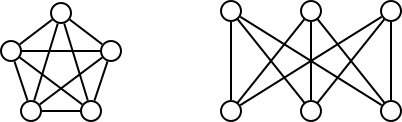
\includegraphics[width=0.8\linewidth]{img/k33andk5.png}
	\caption{A sx il grafo $k_5$, a dx il grafo $k_{3,3}$.}
	\label{fig:graphk5,k33}
\end{figure}

\begin{figure}[h]
	\centering
	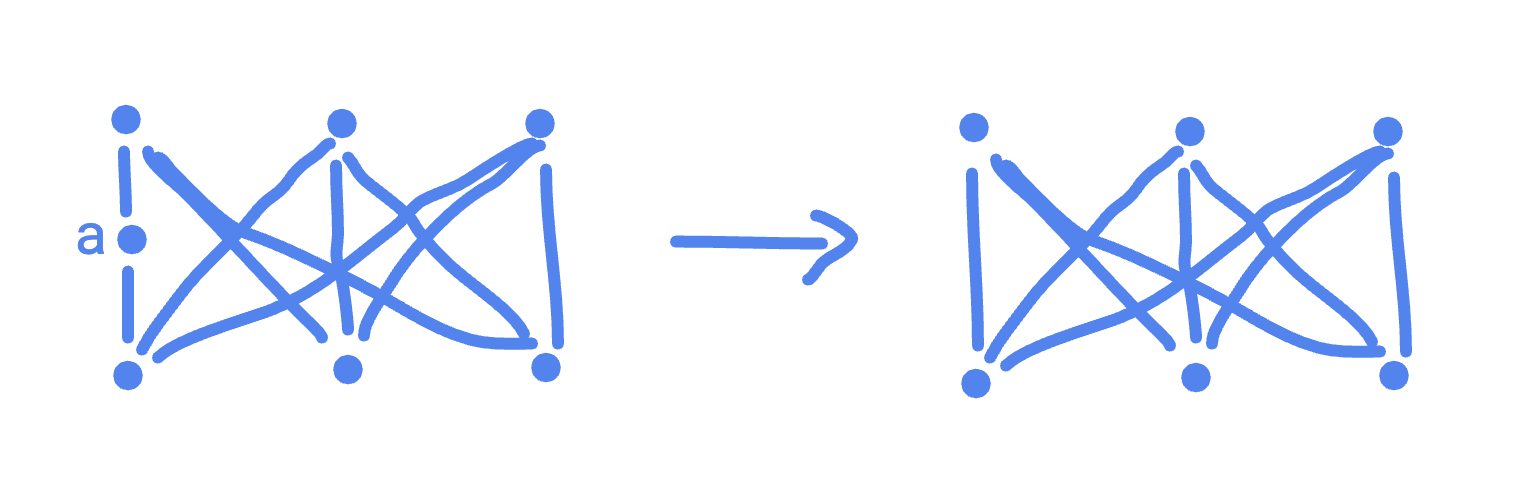
\includegraphics[width=0.8\linewidth]{img/subdivision}
	\caption{Supponendo che il disegno a sx sia una parte del grafo originale, allora rimuovendo il vertice $a$, collegando i due archi che prima erano separati proprio dal vertice $a$, otteniamo il grafo $k_{3,3}$, questo significa quindi che il sotto grafo a sx è un subdivision di $k_{3,3}$, ossia che il grafo originale non è planare.}
	\label{fig:graphk5,k33}
\end{figure}

\subsection{Planarity testing}
Il teorema di Kuratowski  afferma una condizione sufficiente affinché un grafo sia planare, ci sono però altre proprietà che riguardano i grafi planari: queste sono basate su: $e$ (edges), $v$ (vertices), $f$ (faces):
\begin{itemize}
\item $e \leq 3v - 6$
\item Sappiamo anche che se nel grafo non ci sono cicli di lunghezza $3$, allora la condizione $e \leq 2v - 4$ è soddisfatta.
\item $f \leq 2v - 4$
\item $v - e + f = 2$
\item Si noti che se un grafo è planare allora sicuramente le condizioni elencate saranno vere, al contrario, non basta verificare che tutte le condizioni siano vere per affermare che un grafo sia planare (sono necessarie ma non sufficienti); si noti anche che queste condizioni mettono principalmente in relazione gli archi con i vertici, infatti un grafo planare tende a essere sparso, ossia il numero di archi viene limitato dal numero di vertici ($E = \bigcirc (V)$)
\end{itemize}

\subsection{Jordan curve theorem}
Questo teorema afferma che: una qualsiasi curva di Jordan, ossia una semplice curva chiusa, divide il piano in una regione interna alla curva ed una regione esterna alla curva; quindi, ogni path che collega un punto di una regione con un punto della regione opposta, dovrà necessariamente intersecare la curva di Jordan.

\subsection{Alcuni algoritmi}
\begin{itemize}
\item \textbf{Path addition}: Questo algoritmo, di Hopcroft-Tarjan, è il primo ad aver mostrato che planarity può essere verificato in tempo lineare rispetto alla dimensione del grafo, possiamo vedere una bozza dell'algoritmo in figura \ref{fig:path_add}.
\item \textbf{Vertex addition}: l'idea è simile a quella di path addition, solo che al posto di considerare una componente del grafo, si considera un vertice alla volta; per implementare questa tecnica sono usate strutture dati particolari tipo pq-trees.
\item \textbf{Edge addition}: simile a vertex addition, ma si considerano gli archi invece che i vertici.
\item \textbf{Construction sequence}: si considerano blocchi di grafi (planari) più complessi rispetto ai precedenti, quindi li si aggancia al pezzo originale, quindi si ripete.
\end{itemize}
L'algoritmo generico che abbiamo visto per planarity può essere semplificato tramite una left to right DFS, quindi, per ogni arco si deve scegliere se posizionarlo a sx o a dx, questa variazione rende l'algoritmo visto, uno dei più efficienti.

\begin{figure}[h]
	\centering
	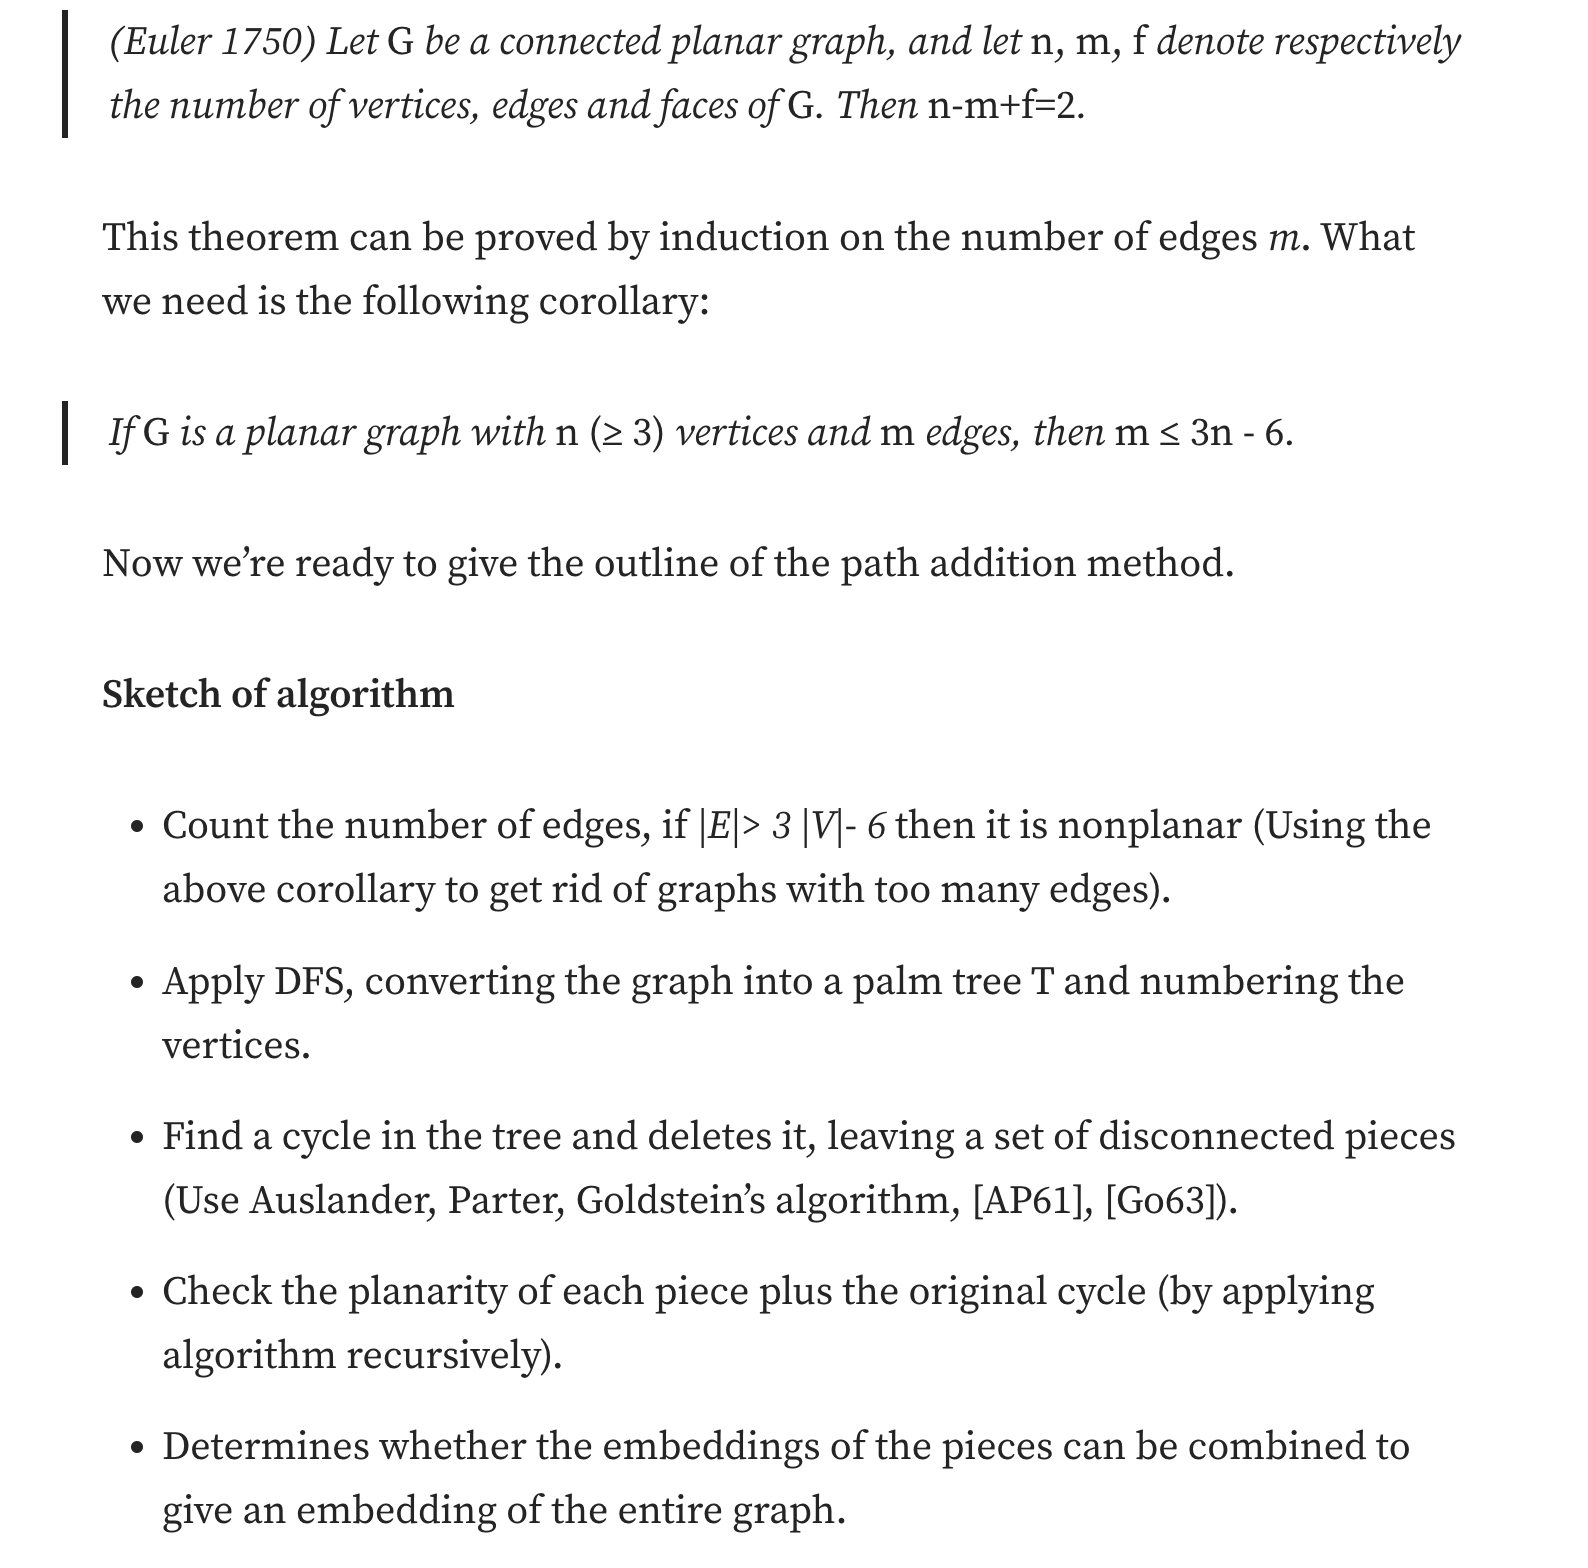
\includegraphics[width=1\linewidth]{img/path_add.png}
	\caption{La schematizzazione dell'algoritmo path addition di Hopcroft-Tarjan}
	\label{fig:path_add}
\end{figure}

\end{document}
